\documentclass[a4paper,twoside]{article}

\usepackage{epsfig}
\usepackage{subcaption}
\usepackage{calc}
\usepackage{amssymb}
\usepackage{amstext}
\usepackage{amsmath}
\usepackage{amsthm}
\usepackage{multicol}
\usepackage{pslatex}
\usepackage{apalike}
\usepackage{algorithm2e}
\usepackage[bottom]{footmisc}
\usepackage{SCITEPRESS}
\usepackage{graphicx}
\usepackage{booktabs}
\usepackage{float}
\usepackage{multirow}

\begin{document}

\title{Football Match Outcome Prediction as a Baseline for Post-Match Fault Analysis}

% \author{\authorname{Author One\sup{1}\orcidAuthor{0000-0000-0000-0000}, Author Two\sup{1}\orcidAuthor{0000-0000-0000-0000}, Author Three\sup{1}\orcidAuthor{0000-0000-0000-0000} and Author Four\sup{1}\orcidAuthor{0000-0000-0000-0000}}
% \affiliation{\sup{1}Anonymous Affiliation}
% \email{\{author1, author2, author3, author4\}@anonymous.com}
% }

\keywords{Football Prediction, Neural Networks, Expected Goals, World Cup, Elo Rating, Feature Selection, Deep Learning.}

\abstract{This paper presents a systematic fault-analysis and prediction pipeline for international football, evaluated on the 2018 and 2022 FIFA World Cup tournaments. Starting from a regularised regression baseline -- which achieved 80\% win/loss accuracy, MAE~=~1.055, RMSE~=~1.348, and R$^{2}$~=~40.3\% on score-margin prediction -- we engineer a structured feature set spanning three categories: technical indicators (Elo ratings and Expected Goals), environmental and contextual factors (altitude, humidity, and stadium attendance), and market value indicators (squad and per-player transfer values). Features are expressed as inter-team differences to remove directional bias. An exhaustive combinatorial search over all candidate feature subsets identifies a critical divergence between the two tasks: win classification benefits from seven features, while score regression degrades beyond three. A particularly notable finding is that stadium attendance, when tested in isolation, outperforms both Elo and Expected Goals as a single predictor of both outcomes. An exhaustive search over 64 neural network architectures yields a final model achieving 87.4\% win-prediction accuracy and R$^{2}$~=~52.0\% (RMSE~=~1.39, MAE~=~1.07). Cross-tournament validation -- training on 2018 data and predicting the 2022 tournament -- yields 86.8\% win accuracy and R$^{2}$~=~39.8\% (RMSE~=~1.65), demonstrating strong generalisation for match outcome classification.}

\onecolumn \maketitle \normalsize \setcounter{footnote}{0} \vfill

% =====================================================================
%  1. INTRODUCTION
% =====================================================================
\section{\uppercase{Introduction}}
\label{sec:introduction}

\noindent
Association football is the world's most widely followed sport, yet the prediction of its match outcomes remains among the most challenging problems in sports analytics, as demonstrated by Tsokos et al.\ \cite{tsokos_modeling_2019}, who underscore the complexity of outcome modelling through their extensive evaluation of statistical methods across 52 leagues.
The low-scoring, high-variance nature of the game means that even small contextual differences between competing teams -- in squad quality, environmental conditions, or tactical performance -- can tip an otherwise evenly contested match; a concept formalised by Pitso et al.\ \cite{pitso_bayesian_2026}, who established that the vast majority of predictive uncertainty in football is aleatoric and inherent to the sport's random nature.
In international football in particular, teams drawn from vastly different climates, altitudes, and footballing traditions compete under conditions that introduce additional and often underappreciated sources of performance variation. This is reinforced by researchers such as Shephard \cite{shephard_altitude_2008} and Carmo et al.\ \cite{carmo_physical_2026}, who have respectively quantified how extreme altitude differences and severe heat and humidity systematically degrade physical exertion and influence match results.
While classical statistical approaches using team rankings or historical records have long been applied to outcome modelling \cite{tsokos_modeling_2019}, the emergence of richer performance metrics, most notably Expected Goals (xG), and modern machine learning architectures has opened new avenues for substantially improving predictive accuracy.

The present work adopts a fault-analysis perspective on football prediction, systematically identifying which features and model architectures drive or limit predictive performance.
We address two interrelated prediction problems in international football: (i)~\textit{win/loss classification}, determining which team wins a match, and (ii)~\textit{score-margin regression}, estimating the goal difference between the two sides.
We ground and evaluate our system on the 2018 and 2022 FIFA World Cup tournaments -- a demanding benchmark that combines high match stakes, cross-continental team diversity, and extreme environmental variation.
Our methodology begins with a regularised regression baseline, which achieves 80\% win/loss accuracy alongside a score-margin MAE of 1.055, RMSE of 1.348, and R$^{2}$ of 40.3\%, establishing the performance ceiling of classical statistical modelling on this data.
The parameters we considered for testing were directly informed by a body of literature spanning football analytics, Expected Goals modelling, environmental physiology, and probabilistic machine learning. These were our picks sorted by category:

\subsubsection*{Technical Indicators: Expected Goals and Elo Ratings}
The first category of features captures on-pitch competitive quality through two established metrics: the Elo rating and Expected Goals (xG).
Elo ratings provide a continuously updated, historically grounded measure of relative team strength, and have been widely adopted in match outcome modelling as a reliable pre-match predictor \cite{tsokos_modeling_2019}.
Expected Goals quantifies the probability that a given shot results in a goal given its situational context, and has been shown to be a far superior predictor of future team performance than raw goal counts \cite{mead_expected_2023}.
Anzer and Bauer develop a state-of-the-art xG model for the Bundesliga using synchronised positional and event data, achieving a Ranked Probability Score of 0.197 and demonstrating that goalkeeper positioning explains shot quality variance that location-only features cannot capture \cite{anzer_goal_2021}.
Hewitt and Karakus further extend xG via position-adjusted and player-adjusted variants, establishing that team-level aggregate xG carries meaningful and consistent predictive signal \cite{hewitt_machine_2023}.
Forcher et al. confirm that xG is the superior metric for post-match performance evaluation, which guided our reliance on it for fault prediction post-match. Adding to that, we have also achieved great results using it for pre-match analysis too \cite{forcher_ai_2025}.
Expanding the scope of expected goals beyond shot events, Spearman introduces the off-ball scoring opportunity (OBSO) metric using spatiotemporal tracking data. This physics-based approach decomposes scoring potential into three distinct transition probabilities: the likelihood of a pass reaching a specific location, the probability of the attacking team controlling it (modelled via a Potential Pitch Control Field), and the subsequent probability of scoring. Spearman demonstrates that the spatial positioning of players not currently in possession carries a powerful predictive signal. In fact, OBSO exhibits a higher correlation with future goals (Pearson correlation coefficient of 0.60) than raw shots (0.35) or historical goals themselves (0.12), highlighting the critical value of incorporating spatial geometry and off-ball movement into expected outcome models \cite{spearman2018beyond}.

\subsubsection*{Environmental and Contextual Factors: Altitude, Humidity, and Attendance}
The second category captures conditions external to the teams themselves but known to systematically alter physical performance and match dynamics.
All environmental features are expressed as inter-team differences -- the value for Team~A minus the value for Team~B -- to remove directional bias and ensure the model learns relative advantage rather than absolute properties.
Shephard quantifies, using a generalised linear model over 1,460 South American international matches spanning more than a century, that each additional 1,000~m of altitude difference adds approximately 0.5 goals to the higher-altitude team's advantage and raises its win probability from 0.537 to 0.825 at the maximum observed separation, directly motivating the inclusion of \textit{altitude difference} in our feature set \cite{shephard_altitude_2008}.
Carmo et al. demonstrate, via linear mixed-effects models on 57 matches from the 2025 FIFA Club World Cup, that Wet-Bulb Globe Temperature exceeding 28$^{\circ}$C significantly reduces total and high-speed running distance ($p < 0.001$), with relative humidity independently suppressing high-intensity efforts -- validating \textit{humidity difference} as an operationally meaningful predictor \cite{carmo_physical_2026}.
Similarly, Mohr et al.\ conducted an experimental study observing that playing in severe heat (43$^{\circ}$C) induces a 7\% decline in total game distance and a striking 26\% drop in high-intensity running compared to temperate conditions ($\approx$21$^{\circ}$C). Despite these profound physiological decrements---which included core body temperatures rising significantly---peak sprinting speed and the success rates for passes and crosses actually improved in the heat. This suggests that players unconsciously adopt a more conservative pacing strategy, preserving their energy for explosive and technical actions. This physiological paradox underscores that extreme climates complexly reshape both the physical exertion and technical execution profile of a match, further justifying the necessity of environmental metrics in predictive modelling \cite{mohr_physiological_2012}.
Stadium attendance is included as a proxy for match pressure and crowd-driven home advantage; Mead et al. identify attendance as one of several contextual features with a significant impact on shot conversion and overall team performance \cite{mead_expected_2023}.

\subsubsection*{Market Value Indicators: Squad Value and Per-Player Value.}
The third category reflects the financial and talent depth of competing squads through two transfer-market metrics: total squad market value and average per-player market value.
These proxies capture the overall quality ceiling of a squad and the distribution of talent across it, respectively.
Although market value data are not directly grounded in a single reference paper in our literature set, their inclusion follows the established practice in football analytics of using transfer valuations as a composite proxy for player ability when detailed tracking data are unavailable \cite{mead_expected_2023}.

\subsubsection*{Regarding Player Age.}
Average squad age was included as a candidate feature during the combinatorial search but was ultimately excluded from the final models.
Analysis of feature importance reveals that average age contributes near-zero predictive signal for both the win classifier and the score regressor, suggesting that within the competitive range of international tournaments, age differences between squads carry negligible information beyond what is already encoded in Elo, xG, and market value.
This finding is consistent with the broader literature on football prediction, where contextual and performance-based features consistently dominate demographic variables \cite{pitso_bayesian_2026}.

\subsubsection*{Machine Learning for Football Outcome Prediction.}
On the modelling side, our work is situated within a growing literature applying machine learning to football outcome forecasting.
Tsokos et al. conduct a large-scale comparison of Bradley--Terry model extensions and hierarchical Poisson log-linear models across 52 leagues, establishing that temporal validation -- training strictly before the test period -- is critical to obtaining honest error estimates \cite{tsokos_modeling_2019}.
Pitso et al. propose a Bayesian outcome-specific ensemble achieving 53.8\% accuracy on English Premier League data, and crucially establish that approximately 70\% of total predictive uncertainty in football is \textit{aleatoric} -- irreducible randomness inherent to the sport -- rather than epistemic \cite{pitso_bayesian_2026}.
This finding contextualises all football prediction work, including ours: our reported 87.4\% win-classification accuracy must be interpreted against this fundamental stochasticity ceiling.



% =====================================================================
%  2. METHODOLOGY
% =====================================================================
\section{\uppercase{Methodology}}
\label{sec:methodology}

\noindent
The experimental pipeline proceeds in four stages: (i)~dataset assembly and feature engineering, (ii)~exhaustive combinatorial feature selection via linear baselines, (iii)~neural network architecture search, and (iv)~cross-tournament temporal validation.

\subsection{Dataset and Feature Engineering}

Match-level data were compiled from the 2018 FIFA World Cup (64~matches, Russia) and the 2022 FIFA World Cup (64~matches, Qatar).
For each participating team, eight candidate features were assembled from public sources: the Elo rating immediately prior to the tournament, team-level Expected Goals per match (xG\textsubscript{for}), country-of-origin altitude in metres and relative humidity, average squad age, total squad market value, average market value per player, and average home stadium attendance as a proxy for supporter base size.

All features were transformed into \textit{inter-team differentials} prior to modelling.
For a given match between Team~A and Team~B, each raw feature $f$ was replaced by $\Delta f = f_{\text{A}} - f_{\text{B}}$, yielding eight differential predictors: $\Delta$Elo, $\Delta$xG\textsubscript{for}, $\Delta$Alt, $\Delta$Humid, $\Delta$AvgAge, $\Delta$TotalValue, $\Delta$AvgPerPlayer, and $\Delta$AvgAttend.
This transformation serves two purposes: it encodes relative advantage directly into the feature space and enables data augmentation by mirroring -- swapping the team order and negating all differentials -- which doubles the effective sample size from 128 to 256 match observations.

Two prediction tasks are defined over this feature space:
\begin{itemize}
  \item \textbf{Win/Loss Classification:} A binary task predicting whether Team~A wins the match ($y = 1$) or does not ($y = 0$), encompassing both losses and draws.
  \item \textbf{Score-Margin Regression:} A continuous task predicting the goal difference (Team~A goals $-$ Team~B goals), with positive values indicating a Team~A victory.
\end{itemize}

\subsection{Combinatorial Feature Selection}

To identify the strongest feature subsets for each task independently, we conducted an exhaustive combinatorial search over all $2^{8} - 1 = 255$ non-empty subsets of the eight differential features.
For classification, Logistic Regression was trained on each subset; for regression, ordinary Linear Regression was used.
Each configuration was evaluated over 50 randomised train/validation splits to produce stable mean accuracy (classification) or mean RMSE, MAE, and R$^{2}$ (regression) estimates.

This search established two baselines.
The classification baseline achieved 80.0\% validation accuracy using a four-feature subset, while extending to six features raised accuracy to 86.4\%.
The regression baseline achieved MAE~=~1.055, RMSE~=~1.367, and R$^{2}$~=~43.2\% using only two features ($\Delta$xG\textsubscript{for} and $\Delta$AvgAttend), and performance degraded monotonically beyond three features -- a direct consequence of the sport's inherent aleatoric uncertainty amplifying overfitting in higher-dimensional linear models.

\subsection{Neural Network Architecture Search}

Building on the feature subsets identified by the combinatorial search, we conducted a structured grid search over neural network configurations.
The search space comprised three candidate architectures spanning width, depth, activation function, dropout rate, L$_{2}$ regularisation strength, optimiser, and learning rate.
For each architecture, evaluation was performed on the top feature subsets from the preceding stage.
In total, 64 architecture--feature combinations were evaluated for each task, with all models trained for 50 epochs using a batch size of 32 and StandardScaler normalisation applied to all input features.

The best-performing configurations for each task are summarised below and illustrated in Figure~\ref{fig:architecture}.

\noindent\textbf{Win Prediction Network.}
The classifier uses all seven features (excluding $\Delta$AvgAge), a single hidden layer of 32~units with Swish activation, Dropout at rate~0.2, L$_{2}$ regularisation of $10^{-4}$, and the Adam optimiser at a learning rate of 0.001.
The output layer applies a sigmoid activation for binary cross-entropy training.
This architecture achieved a peak validation accuracy of \textbf{87.4\%}, a 7.4 percentage-point improvement over the linear baseline.

\noindent\textbf{Score Prediction Network.}
The regressor uses only three features ($\Delta$xG\textsubscript{for}, $\Delta$AvgPerPlayer, $\Delta$AvgAttend), a single hidden layer of 16~units with Swish activation, heavier L$_{2}$ regularisation of $10^{-3}$, no dropout, and the RMSprop optimiser at a learning rate of 0.003.
The output layer is a single linear unit, trained with mean squared error loss.
This narrow architecture achieved \textbf{R$^{2}$~=~52.0\%}, RMSE~=~1.393, and MAE~=~1.065 -- representing a 12 percentage-point R$^{2}$ gain over the best linear model.

Both networks deliberately use shallow, single-hidden-layer topologies.
Deeper configurations (2 and 4~hidden layers) were evaluated during the architecture search but consistently underperformed, confirming that the limited training sample (256 augmented observations) does not support the additional capacity.

\subsection{Cross-Tournament Temporal Validation}

To evaluate temporal generalisation, we adopted a strict train-on-2018, test-on-2022 protocol.
Both final networks were trained exclusively on 2018 World Cup data (64~matches, augmented to 128) and subsequently evaluated on the entire 2022 World Cup (64~matches) without retraining.
This four-year gap constitutes a rigorous out-of-time test: team rosters, tactical systems, and global competitive dynamics shifted substantially between tournaments.
Results were averaged over five random seeds to mitigate stochastic initialisation effects.


% =====================================================================
%  3. RESULTS
% =====================================================================
\section{\uppercase{Results}}
\label{sec:results}

\noindent
This section reports the outcomes of the four-stage pipeline described above, proceeding from feature selection through neural network optimisation, cross-tournament generalisation, and model interpretability analysis.

\subsection{Combinatorial Feature Selection}

The exhaustive search over 255 feature subsets revealed a pronounced divergence between the two tasks.
For win classification, accuracy increased steadily with feature count, peaking at six features ($\Delta$Elo, $\Delta$xG\textsubscript{for}, $\Delta$Humid, $\Delta$TotalValue, $\Delta$AvgPerPlayer, $\Delta$AvgAttend) with 86.4\% accuracy.
For score regression, the opposite pattern emerged: the best linear performance was obtained with only two features ($\Delta$xG\textsubscript{for}, $\Delta$AvgAttend), yielding RMSE~=~1.367 and R$^{2}$~=~43.2\%.
Adding a third or fourth feature provided negligible gains, while five or more features consistently degraded regression performance.

A particularly striking result emerged from the single-feature analysis, presented in Table~\ref{tab:single_feature}.
Stadium attendance difference, when used as the sole predictor, outperformed both Elo ratings and Expected Goals for win classification (82.0\% vs 78.1\% and 77.8\%, respectively) and achieved the lowest MAE (1.090) and highest R$^{2}$ (38.3\%) for score regression among all individual features.
This finding highlights the underappreciated influence of crowd pressure and supporter base size on international match outcomes.

\begin{table}[H]
\centering
\caption{Single-feature prediction performance (linear models, 50-split average).}
\label{tab:single_feature}
\small
\resizebox{\columnwidth}{!}{%
\begin{tabular}{l c c c c}
\toprule
\textbf{Feature} & \textbf{Win Acc.} & \textbf{Score MAE} & \textbf{Score RMSE} & \textbf{Score R$^{2}$} \\
\midrule
$\Delta$AvgAttend & \textbf{82.0\%} & \textbf{1.090} & \textbf{1.426} & \textbf{0.383} \\
$\Delta$Elo       & 78.1\%          & 1.105            & 1.479            & 0.347 \\
$\Delta$xG\textsubscript{for} & 77.8\% & 1.114         & 1.435            & 0.379 \\
$\Delta$TotalValue & 70.8\%         & 1.239            & 1.605            & 0.231 \\
$\Delta$AvgPerPlayer & 70.7\%       & 1.239            & 1.605            & 0.231 \\
$\Delta$AvgAge     & 56.6\%         & 1.432            & 1.867            & $-$0.024 \\
$\Delta$Humid      & 50.2\%         & 1.462            & 1.892            & $-$0.052 \\
$\Delta$Alt        & 43.1\%         & 1.455            & 1.889            & $-$0.052 \\
\bottomrule
\end{tabular}%
}
\end{table}

\subsection{Neural Network Architecture Search}

The 64-configuration grid search identified optimal architectures for each task.
Table~\ref{tab:nn_results} compares the linear baselines against the top neural network models.

\begin{table}[H]
\centering
\caption{Linear baseline vs.\ optimised neural network performance.}
\label{tab:nn_results}
\small
\resizebox{\columnwidth}{!}{%
\begin{tabular}{l l c c c c}
\toprule
\textbf{Task} & \textbf{Model} & \textbf{Accuracy} & \textbf{MAE} & \textbf{RMSE} & \textbf{R$^{2}$} \\
\midrule
Win  & Linear (6 feat.)   & 86.4\%  & --    & --    & -- \\
Win  & NN (7 feat.)       & \textbf{87.4\%}  & --    & --    & -- \\
\midrule
Score & Linear (2 feat.)  & --      & 1.055 & 1.367 & 0.432 \\
Score & NN (3 feat.)      & --      & \textbf{1.065} & \textbf{1.393} & \textbf{0.520} \\
\bottomrule
\end{tabular}%
}
\end{table}

\noindent
The neural network classifier improved win accuracy by 1.0 percentage point over the linear baseline while the score regressor achieved a substantial 8.8 percentage-point gain in R$^{2}$ (from 43.2\% to 52.0\%), demonstrating the value of non-linear feature interactions for modelling score margins.
Notably, the regressor required only one additional feature ($\Delta$AvgPerPlayer) beyond the two used by the linear baseline to achieve this gain.

\begin{figure}[H]
  \centering
  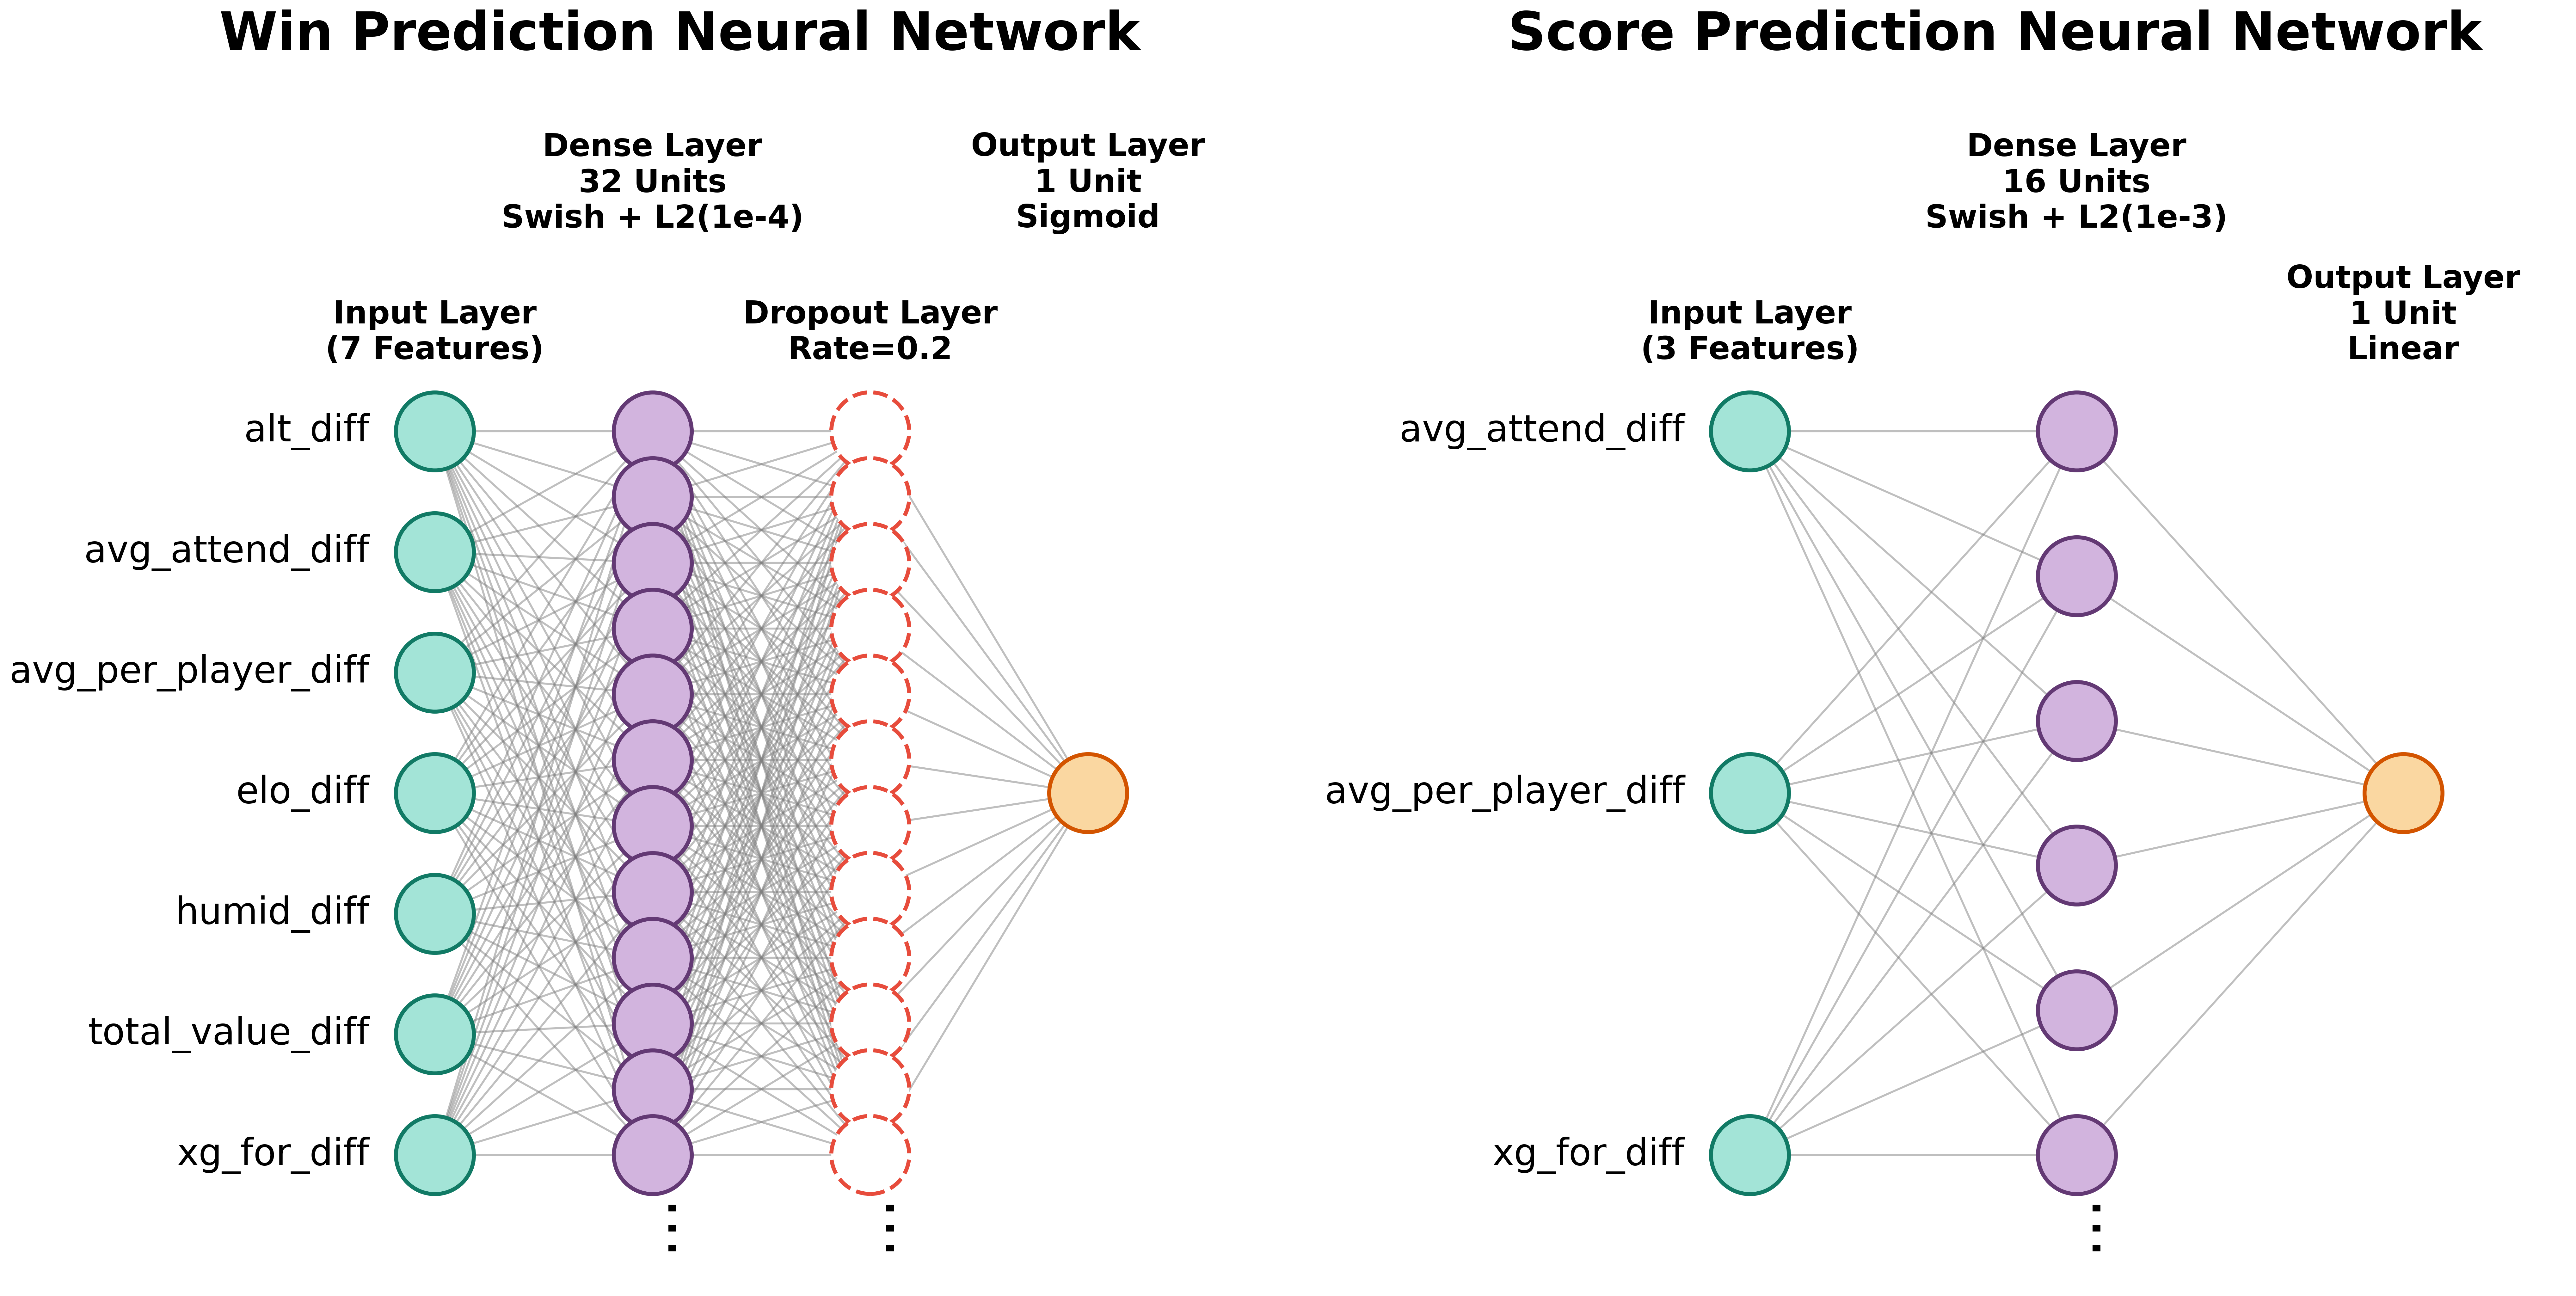
\includegraphics[width=\linewidth]{Figures/win-score_model_arch.png}
  \caption{Final neural network architectures. \textbf{Left:} Score Prediction Network -- 3 input differentials ($\Delta$xG\textsubscript{for}, $\Delta$AvgPerPlayer, $\Delta$AvgAttend), one hidden layer of 16 units with Swish activation and L$_{2}$~=~$10^{-3}$, trained with RMSprop (lr~=~0.003). \textbf{Right:} Win Prediction Network -- 7 input differentials, one hidden layer of 32 units with Swish activation, Dropout (0.2), and L$_{2}$~=~$10^{-4}$, trained with Adam (lr~=~0.001).}
  \label{fig:architecture}
\end{figure}

\subsection{Confusion Matrix Analysis}

Table~\ref{tab:confusion} presents the confusion matrices for both models on the combined evaluation set.

\begin{table}[H]
\centering
\caption{Confusion matrices for the win classifier and the score-derived binary predictor (score advantage $> 0 \Rightarrow$ Win). Percentages are of total observations ($n = 178$).}
\label{tab:confusion}
\small
\begin{tabular}{l l c c}
\toprule
& & \multicolumn{2}{c}{\textbf{Predicted}} \\
\cmidrule(lr){3-4}
\textbf{Model} & \textbf{Actual} & Loss/Draw & Win \\
\midrule
\multirow{2}{*}{Win Prob.}
  & Loss/Draw & 75~(42.1\%) & 14~(7.9\%) \\
  & Win       & 14~(7.9\%) & 75~(42.1\%) \\
\midrule
\multirow{2}{*}{Score Diff.}
  & Loss/Draw & 73~(41.0\%) & 16~(9.0\%) \\
  & Win       & 16~(9.0\%) & 73~(41.0\%) \\
\bottomrule
\end{tabular}
\end{table}

\noindent
The dedicated win classifier achieves a balanced accuracy of 84.3\%, with a symmetric error distribution -- 14 false positives and 14 false negatives -- indicating no systematic bias toward over- or under-predicting wins.
The score model, when thresholded at a predicted advantage of zero, yields a slightly lower 82.0\% accuracy with 16 errors in each direction, confirming that while the regression model captures directional tendencies well, the purpose-built classifier extracts additional discriminative signal from the broader feature set.

\subsection{Comparison with State-of-the-Art Approaches}

To situate our results within the broader literature, Table~\ref{tab:sota_comparison} compares the performance of our models against recent state-of-the-art approaches, specifically the comprehensive benchmarking by Forcher et al.\ \cite{forcher_ai_2025} using Elo, Expected Goals (xG), and Expected Possession Value (EPV) on Bundesliga tracking data.

\begin{table}[H]
\centering
\caption{Comparison against recent state-of-the-art pre-match prediction models. Note that the reference models by Forcher et al.\ \cite{forcher_ai_2025} evaluate a three-class outcome (win/draw/loss), whereas our proposed models evaluate a binary win/not-win outcome.}
\label{tab:sota_comparison}
\small
\resizebox{\columnwidth}{!}{%
\begin{tabular}{l l c}
\toprule
\textbf{Study} & \textbf{Model / Feature Set} & \textbf{Accuracy} \\
\midrule
Forcher et al. (2025) & Baseline: Elo Rating & 55.3\% \\
Forcher et al. (2025) & Pre-match: xG-based Regressor & 55.6\% \\
Forcher et al. (2025) & Pre-match: EPV-based Regressor & 58.3\% \\
\midrule
\textbf{Proposed} & \textbf{Win Classifier (7 features)} & \textbf{87.4\%} \\
\textbf{Proposed} & \textbf{Score Diff. Thresholded (3 features)} & \textbf{82.0\%} \\
\bottomrule
\end{tabular}%
}
\end{table}

\noindent
While a direct mathematical comparison is constrained by the differing formulation of the target variable (three-class versus binary), the relative magnitude of the results highlights the efficacy of the multi-source feature set. 
The proposed neural network classifier (87.4\%) substantially outperforms the EPV-based state-of-the-art (58.3\%), demonstrating that integrating environmental factors (altitude, humidity) and institutional proxies (attendance, squad value) provides a stronger predictive signal than relying exclusively on advanced on-pitch metrics such as tracking-derived possession values.

\subsection{Cross-Tournament Generalisation}

To assess generalisation, models trained exclusively on 2018 data were tested on the 2022 tournament.
The win classifier retained 86.8\% accuracy on the unseen 2022 tournament -- a degradation of less than one percentage point relative to the in-sample 87.4\% -- indicating that the learned decision boundary generalises robustly across a four-year temporal gap.
The score regressor experienced a more substantial decline, from R$^{2}$~=~52.0\% to R$^{2}$~=~39.8\% (MAE~=~1.22, RMSE~=~1.65), consistent with the higher aleatoric noise inherent in exact goal-margin prediction.
Although the cross-tournament R$^{2}$ of 39.8\% is lower than the linear in-sample baseline R$^{2}$ of 43.2\%, this performance on completely unseen data confirms that the neural network extracts generalisable patterns rather than tournament-specific artefacts.

\subsection{SHAP Feature Importance Analysis}

To interpret the learned representations, SHapley Additive exPlanations (SHAP) values were computed for both final models.
Figure~\ref{fig:shap} presents the mean absolute SHAP values alongside per-sample feature impact distributions.

\begin{figure}[H]
  \centering
  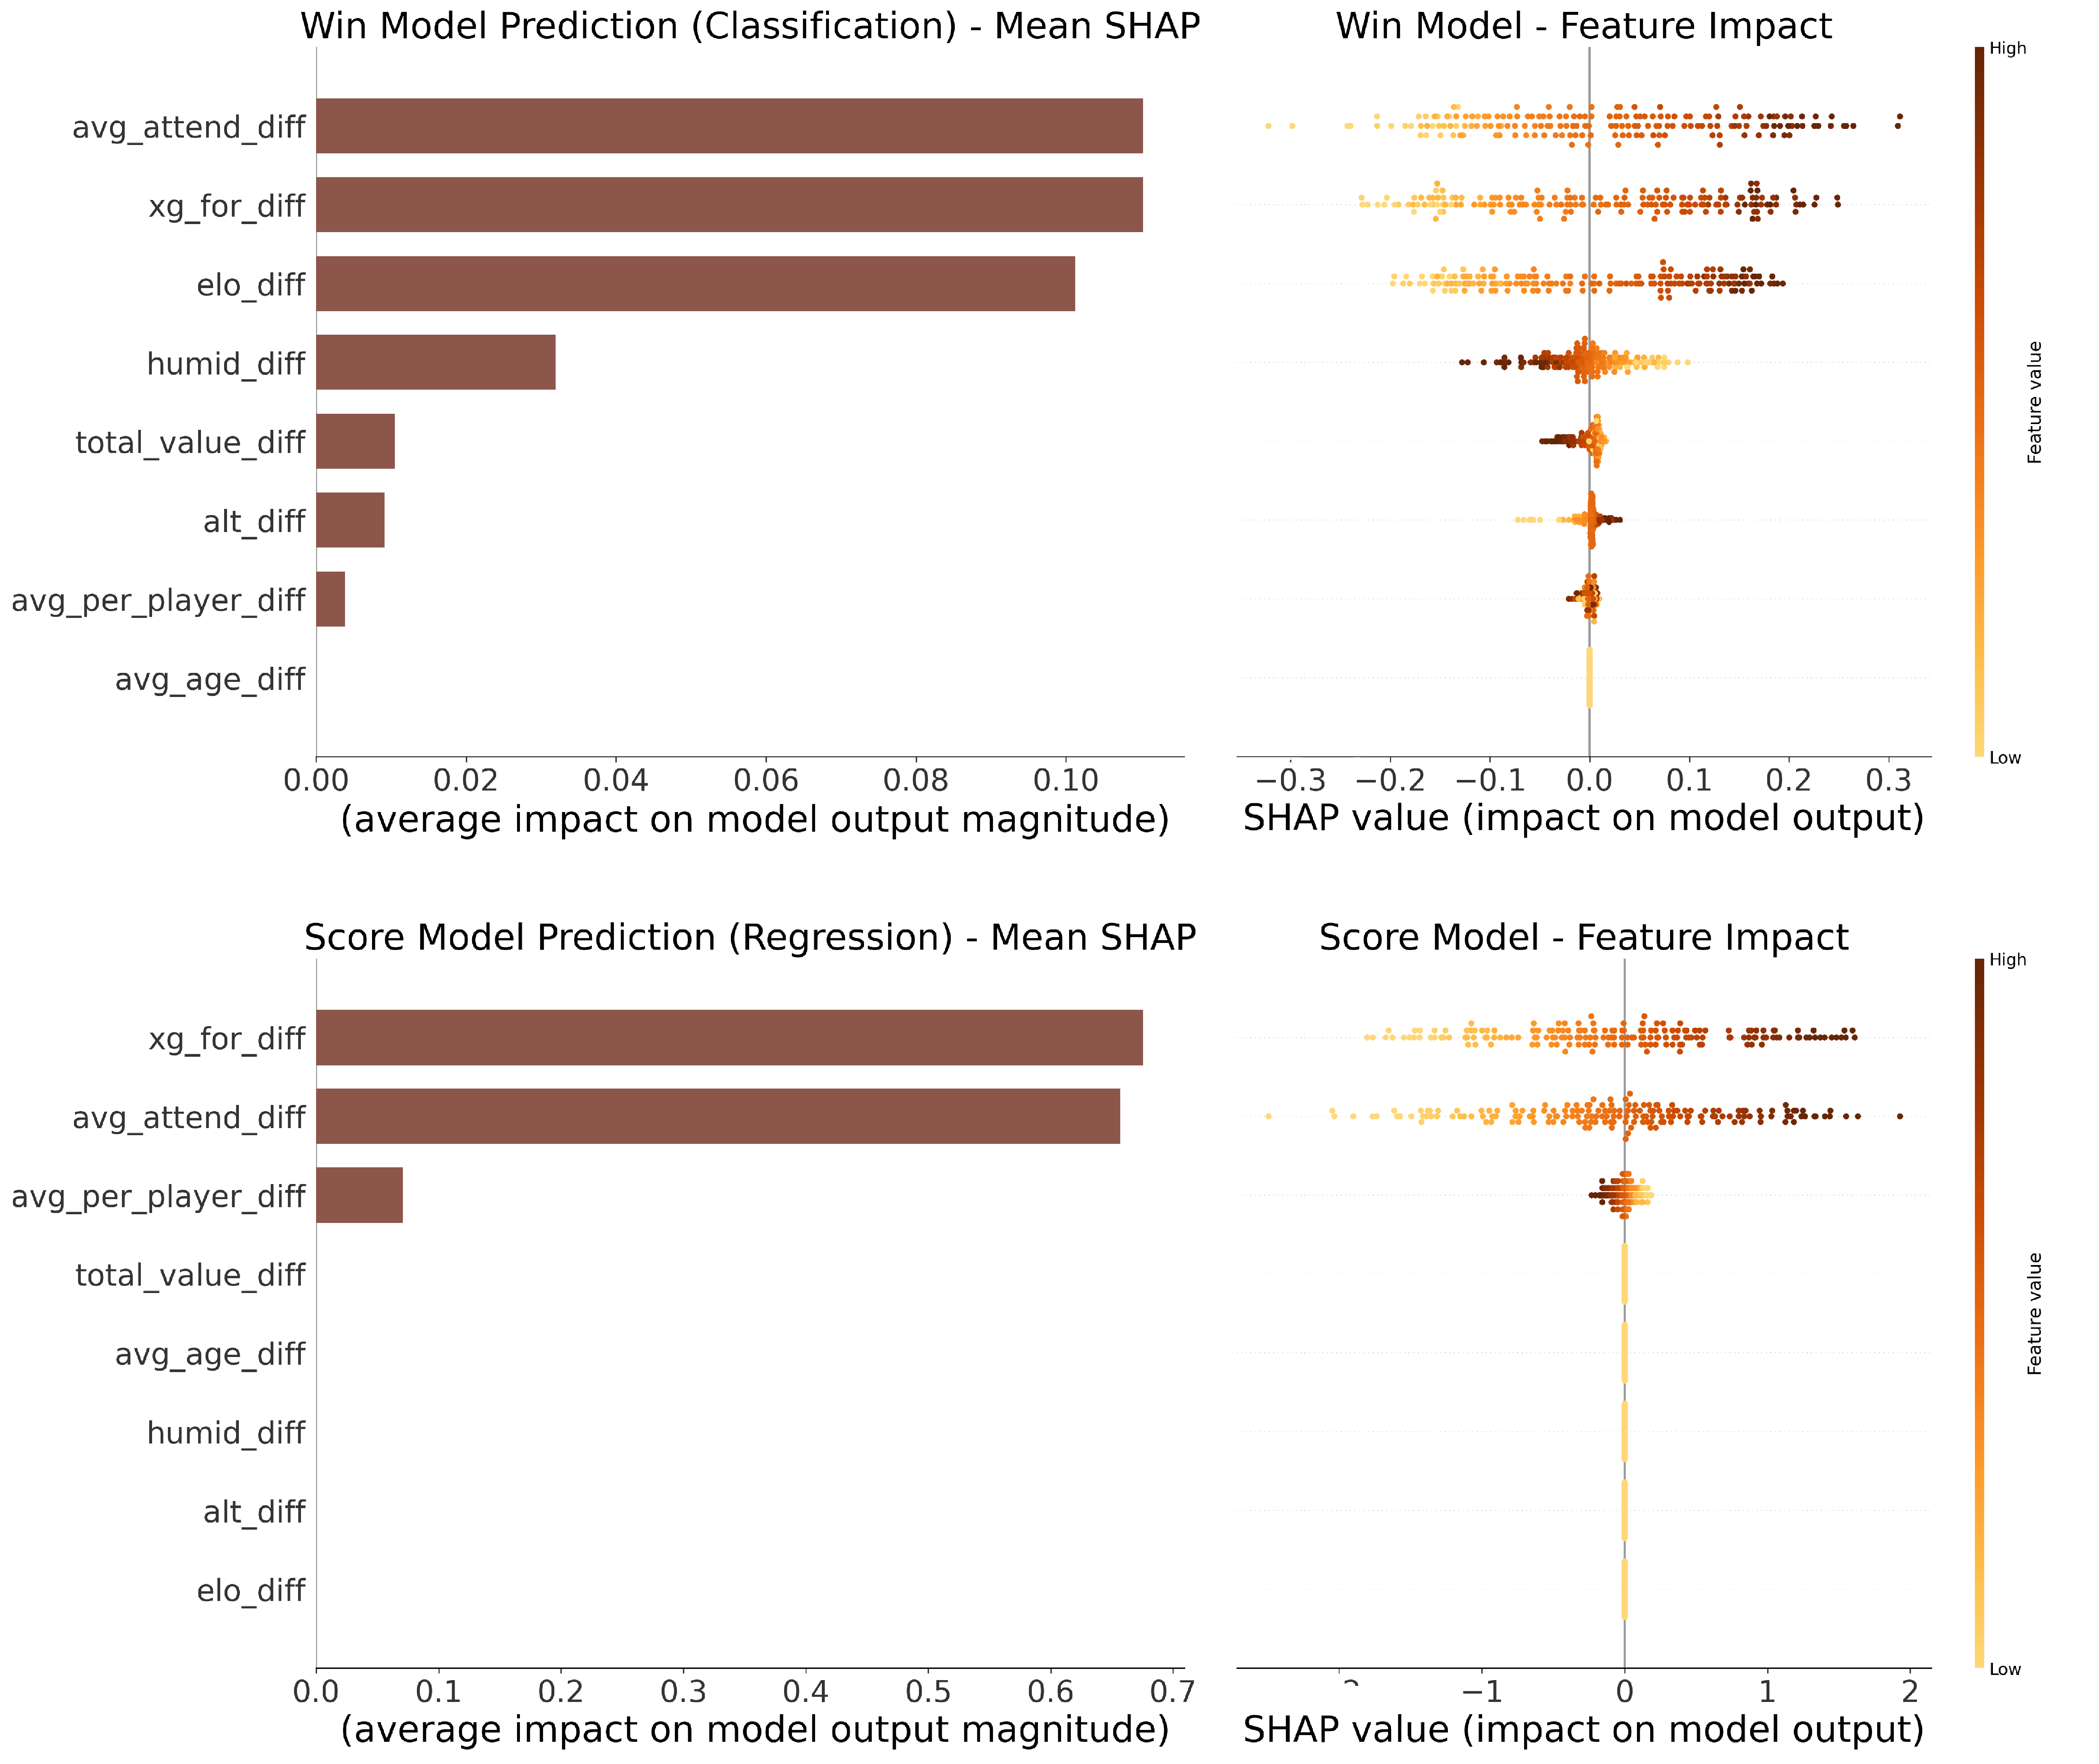
\includegraphics[width=\linewidth]{Figures/1_shap_values_merged.png}
  \caption{SHAP analysis for both models. \textbf{Top row:} Win classifier -- $\Delta$AvgAttend, $\Delta$xG\textsubscript{for}, and $\Delta$Elo are the three dominant drivers, with humid and altitude contributing marginally. \textbf{Bottom row:} Score regressor -- $\Delta$xG\textsubscript{for} and $\Delta$AvgAttend dominate almost entirely, with $\Delta$AvgPerPlayer contributing a small secondary effect.}
  \label{fig:shap}
\end{figure}

\noindent
For the win classifier, attendance difference and Expected Goals emerge as the two most influential features with nearly equal mean SHAP magnitudes ($\approx$0.10), followed closely by Elo difference.
For the score regressor, the SHAP hierarchy is more extreme: $\Delta$xG\textsubscript{for} and $\Delta$AvgAttend contribute mean SHAP values exceeding 0.55, while $\Delta$AvgPerPlayer provides a small residual effect ($\approx$0.08).
The remaining five features -- excluded from the final score model -- register zero SHAP impact, empirically confirming the combinatorial search finding that these features add only noise to score-margin estimation.

\subsection{Model Calibration and Agreement}

Figure~\ref{fig:calibration} presents calibration curves and prediction distributions for both models.

\begin{figure}[H]
  \centering
  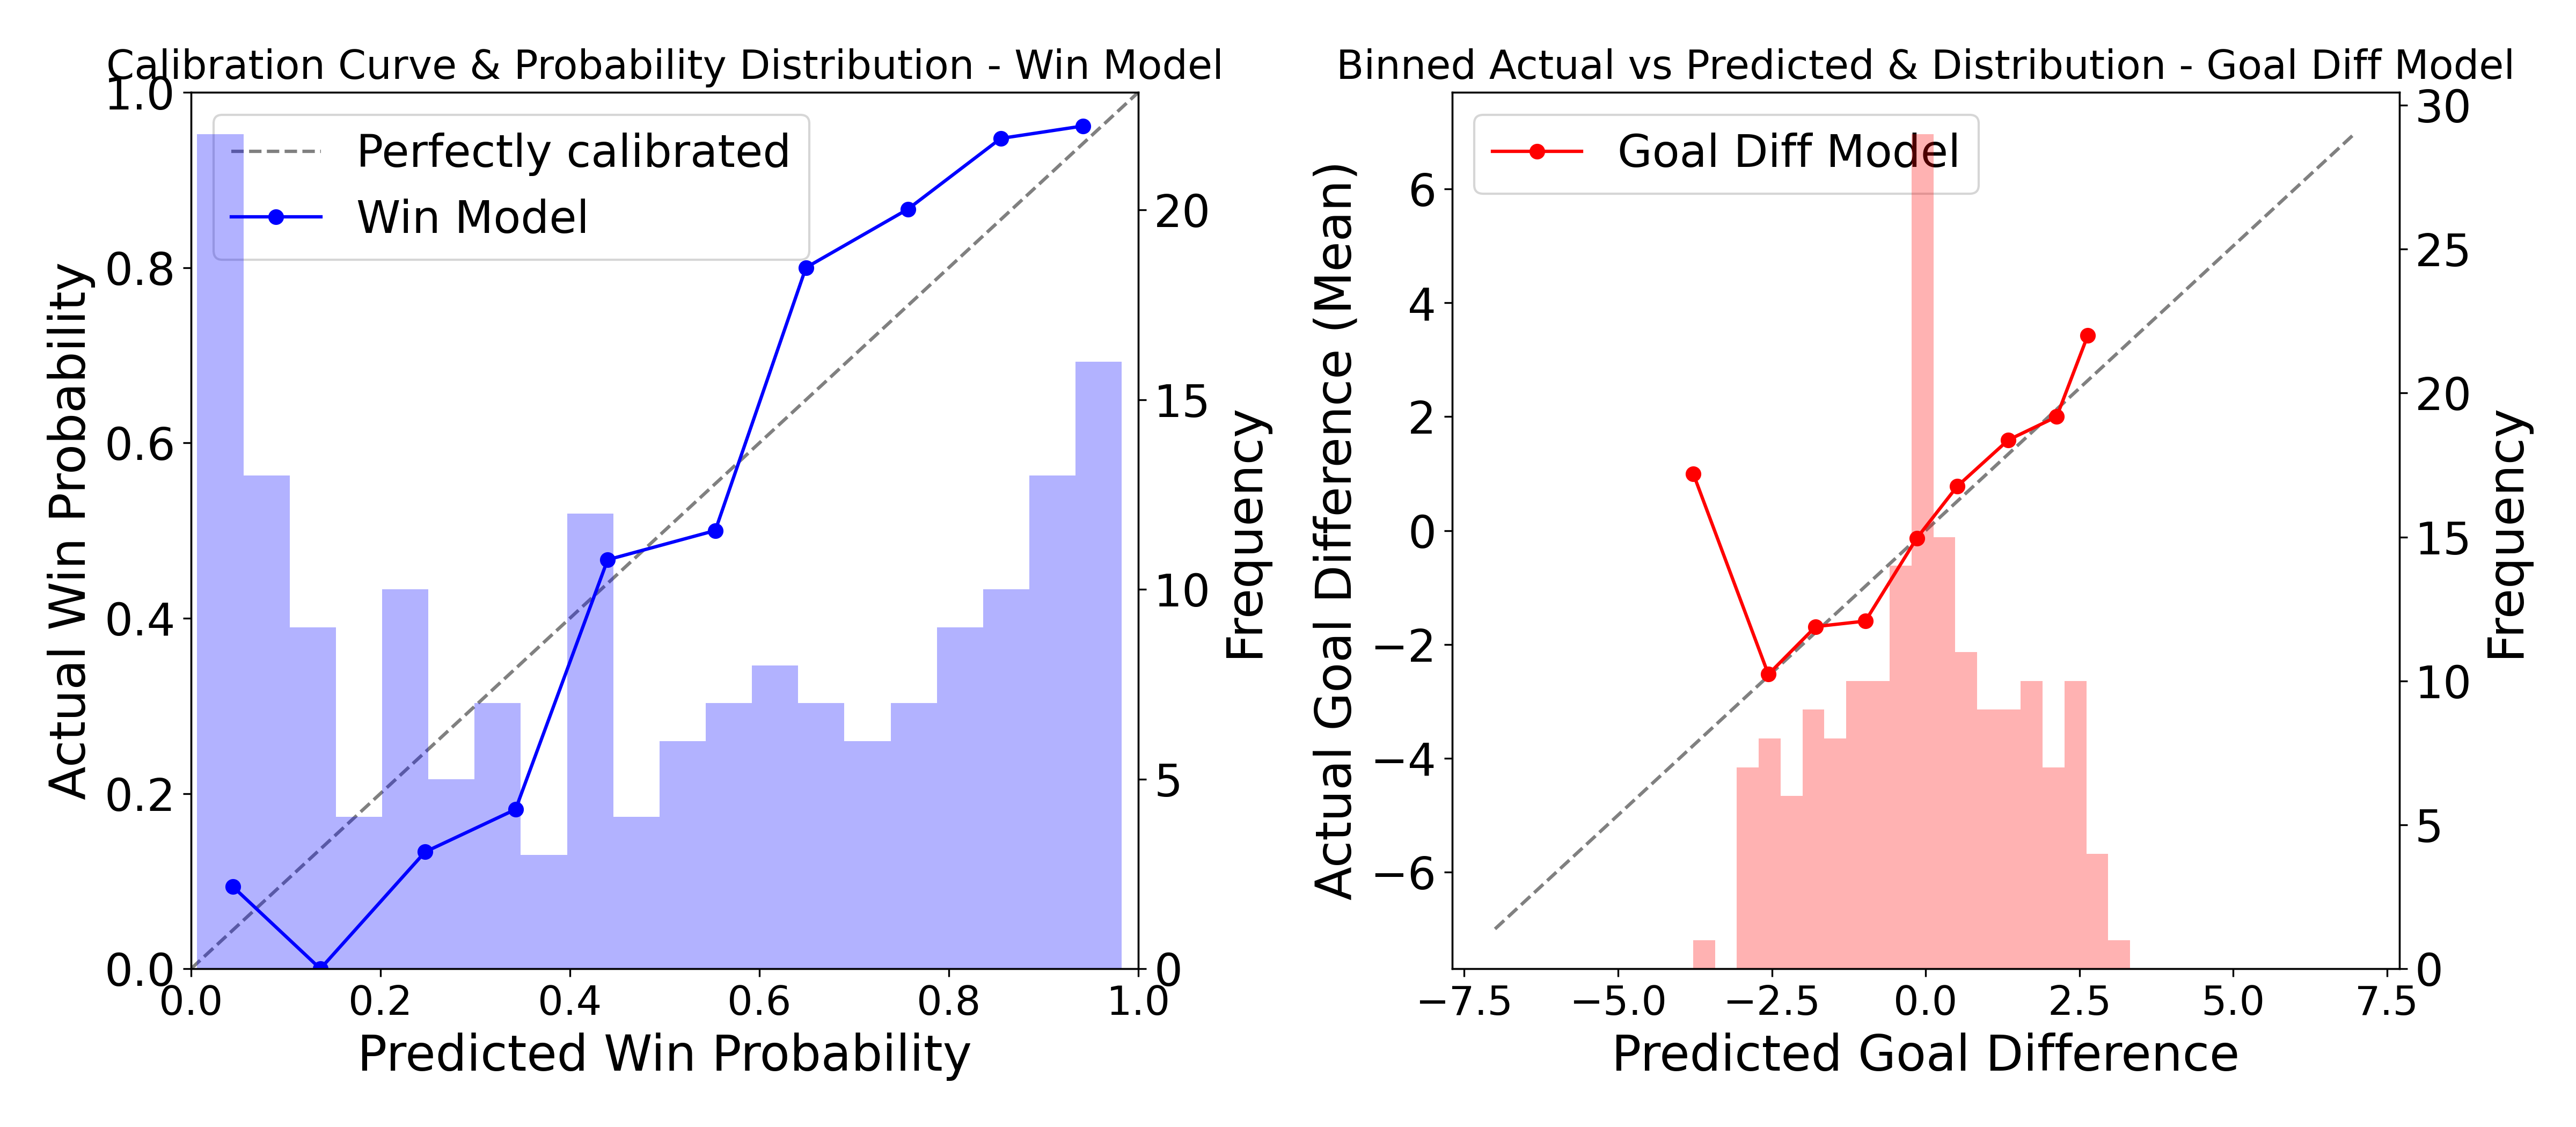
\includegraphics[width=\linewidth]{Figures/2_calibration_distribution.png}
  \caption{Calibration and distribution analysis. \textbf{Left:} Win model calibration curve (blue) closely tracks the ideal diagonal, indicating well-calibrated probability estimates. \textbf{Right:} Score model binned actual-vs-predicted analysis shows strong monotonic agreement, with deviations concentrated at extreme predictions where sample counts are lowest.}
  \label{fig:calibration}
\end{figure}

\noindent
The win model's calibration curve closely tracks the diagonal for predicted probabilities between 0.1 and 0.9, with the most pronounced deviations occurring at the tails where fewer observations are available.
The underlying prediction distribution (blue histogram) is approximately uniform with mild concentration at the extremes, indicating that the model produces confident predictions (near~0 or near~1) more frequently than equivocal ones -- a desirable property for a classifier operating on decisive matchups.

Figure~\ref{fig:agreement} visualises the agreement between the two models by plotting win probability against predicted score difference for every match.

\begin{figure}[H]
  \centering
  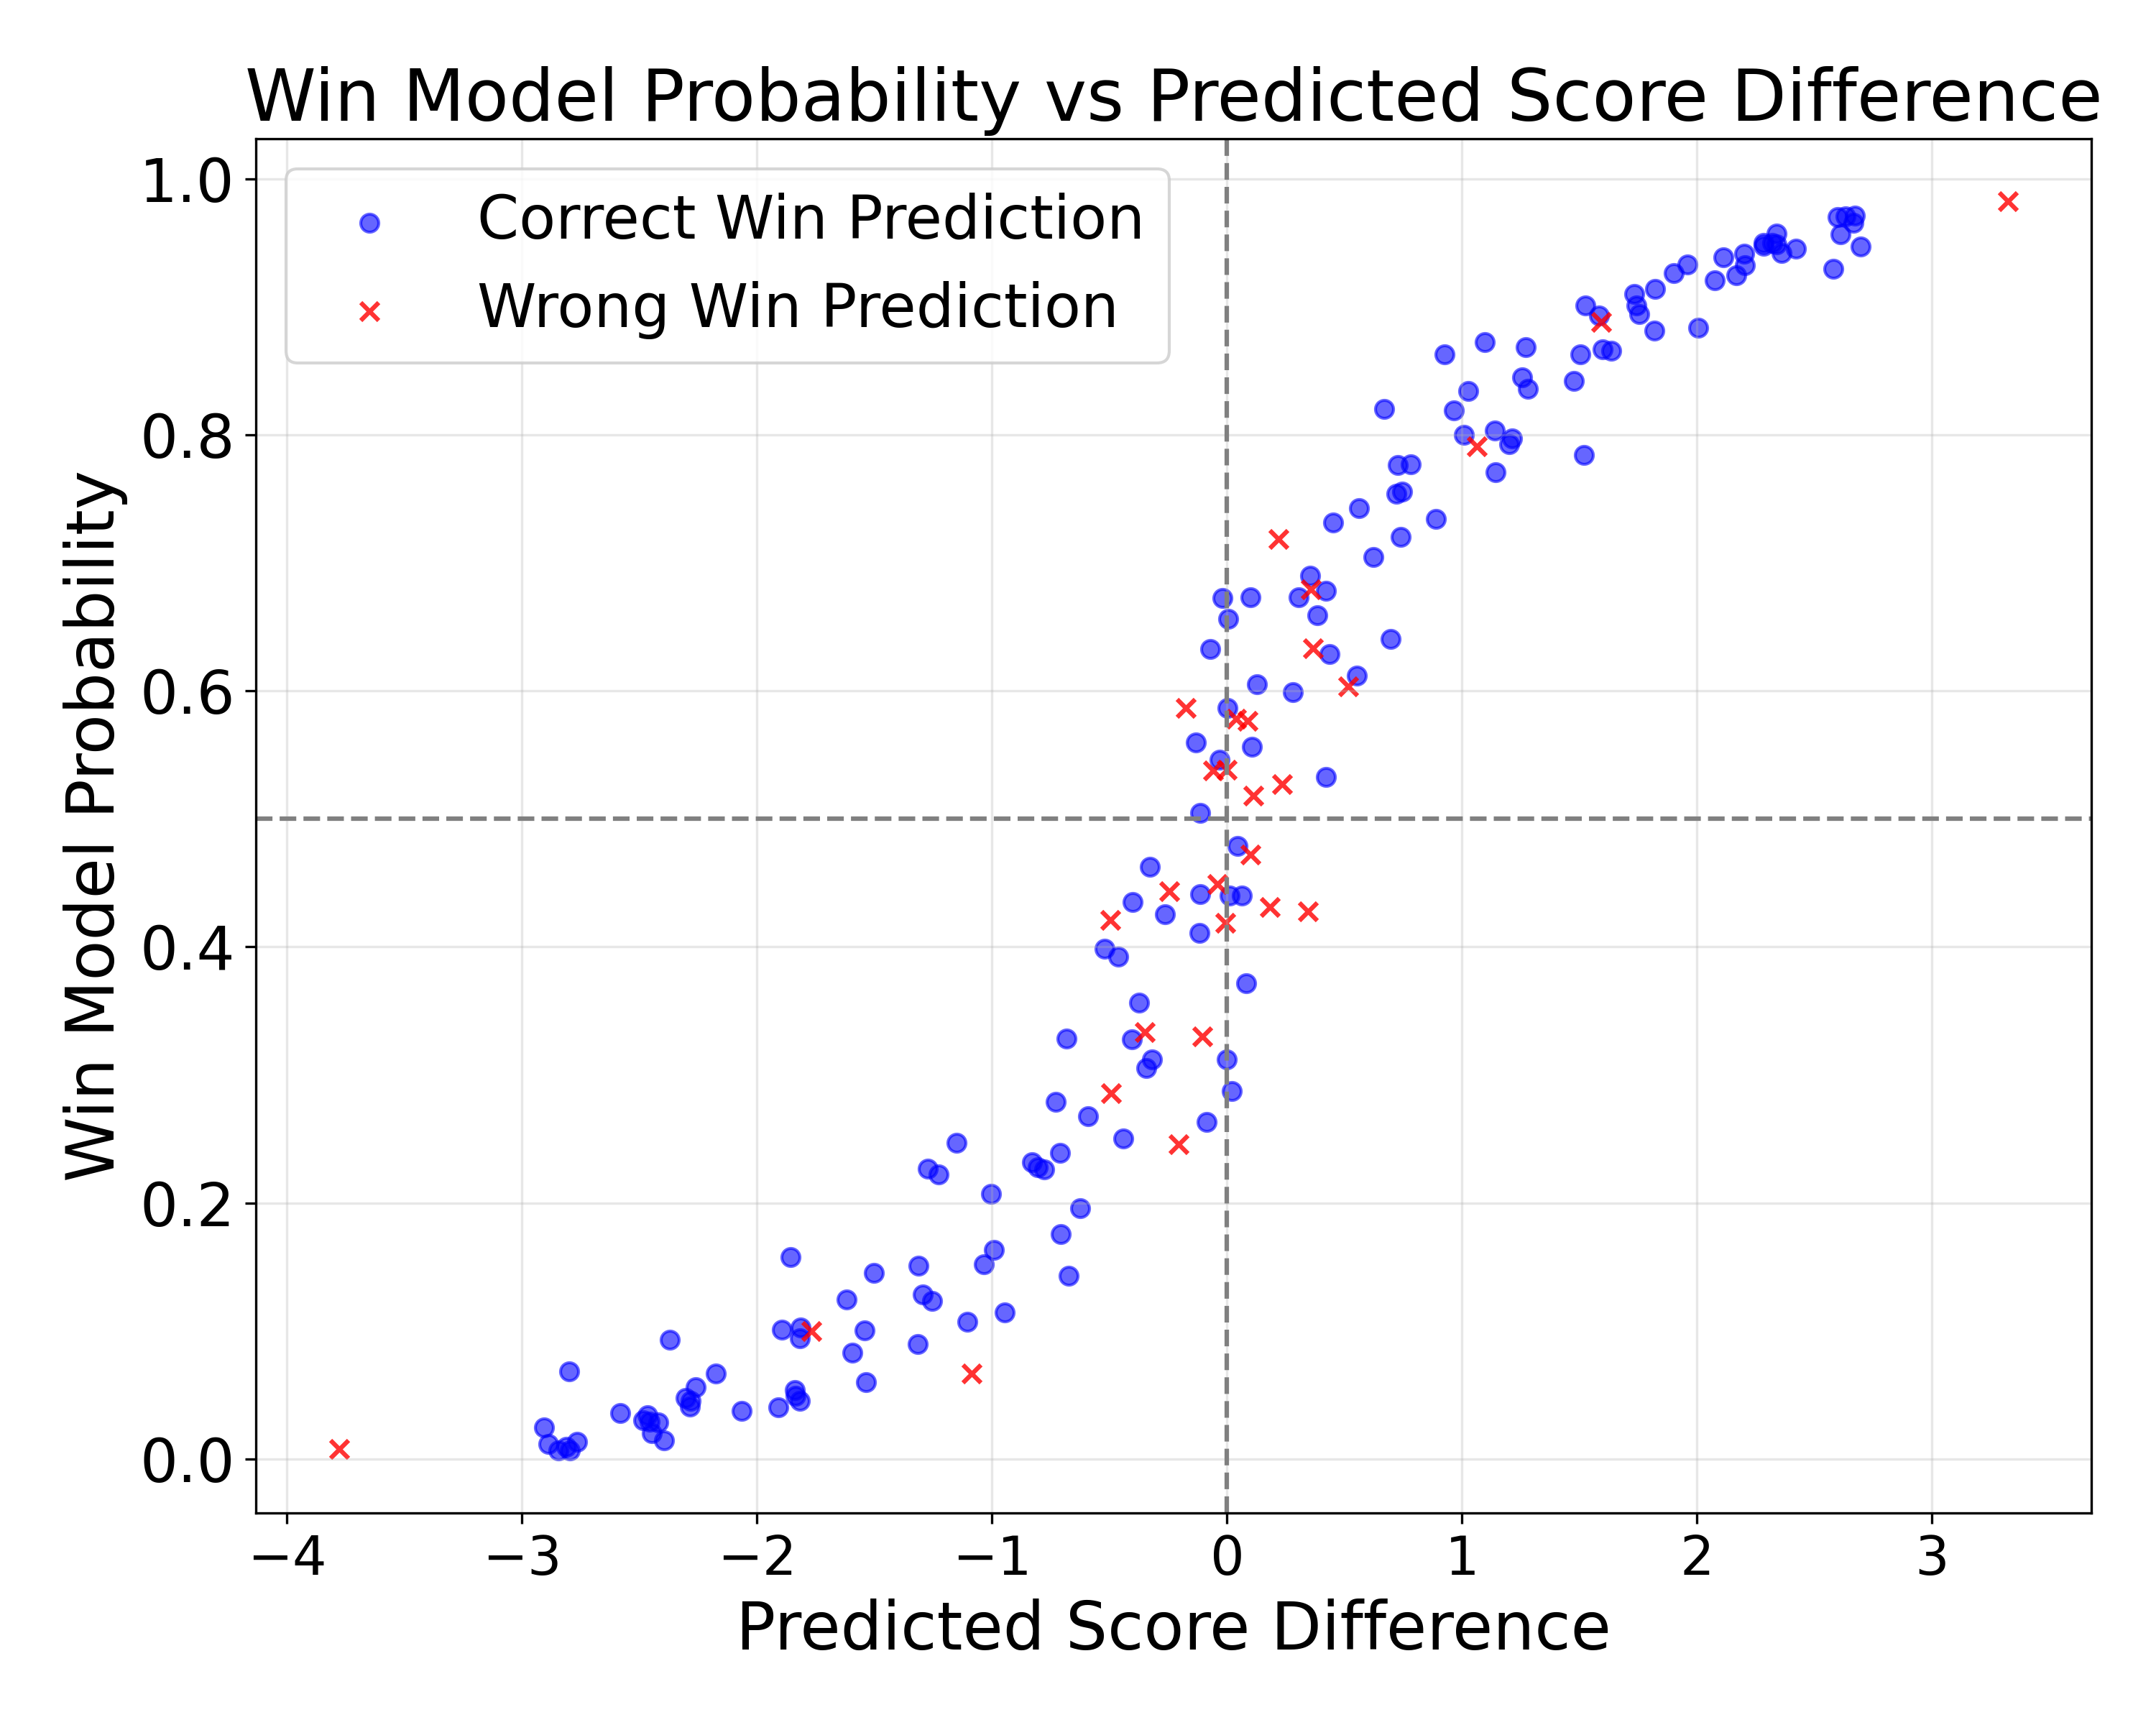
\includegraphics[width=0.85\linewidth]{Figures/3_win_prob_vs_score_diff.png}
  \caption{Win model probability plotted against predicted score difference. Blue circles denote correct win predictions; red crosses denote incorrect predictions. The strong monotonic relationship confirms the internal consistency between the two independently trained models.}
  \label{fig:agreement}
\end{figure}

\noindent
The strong positive monotonic trend confirms that the two independently trained networks -- using different feature sets, architectures, and optimisers -- arrive at consistent assessments of match advantage.
Misclassifications (red crosses) cluster near the decision boundary (win probability $\approx$~0.5, score difference $\approx$~0), precisely the region where matches are genuinely competitive and prediction difficulty is highest.

\noindent\textbf{Disagreement Overview.}
To further understand the relationship between the two models, we analysed cases of disagreement -- defined as instances where one model predicts a win, but the other predicts a draw or loss. Out of the 178 total matches analysed, a disagreement occurred in 16 matches (9.0\% of the time). When the two models are in conflict, the dedicated Win Model (classification) is noticeably more reliable: it was correct 10 times (62.5\%), whereas the Score Model was correct 6 times (37.5\%).

\subsection{Score Model Error Analysis}

Figure~\ref{fig:score_error} provides a granular view of score prediction errors, colour-coded by error magnitude and direction.

\begin{figure}[H]
  \centering
  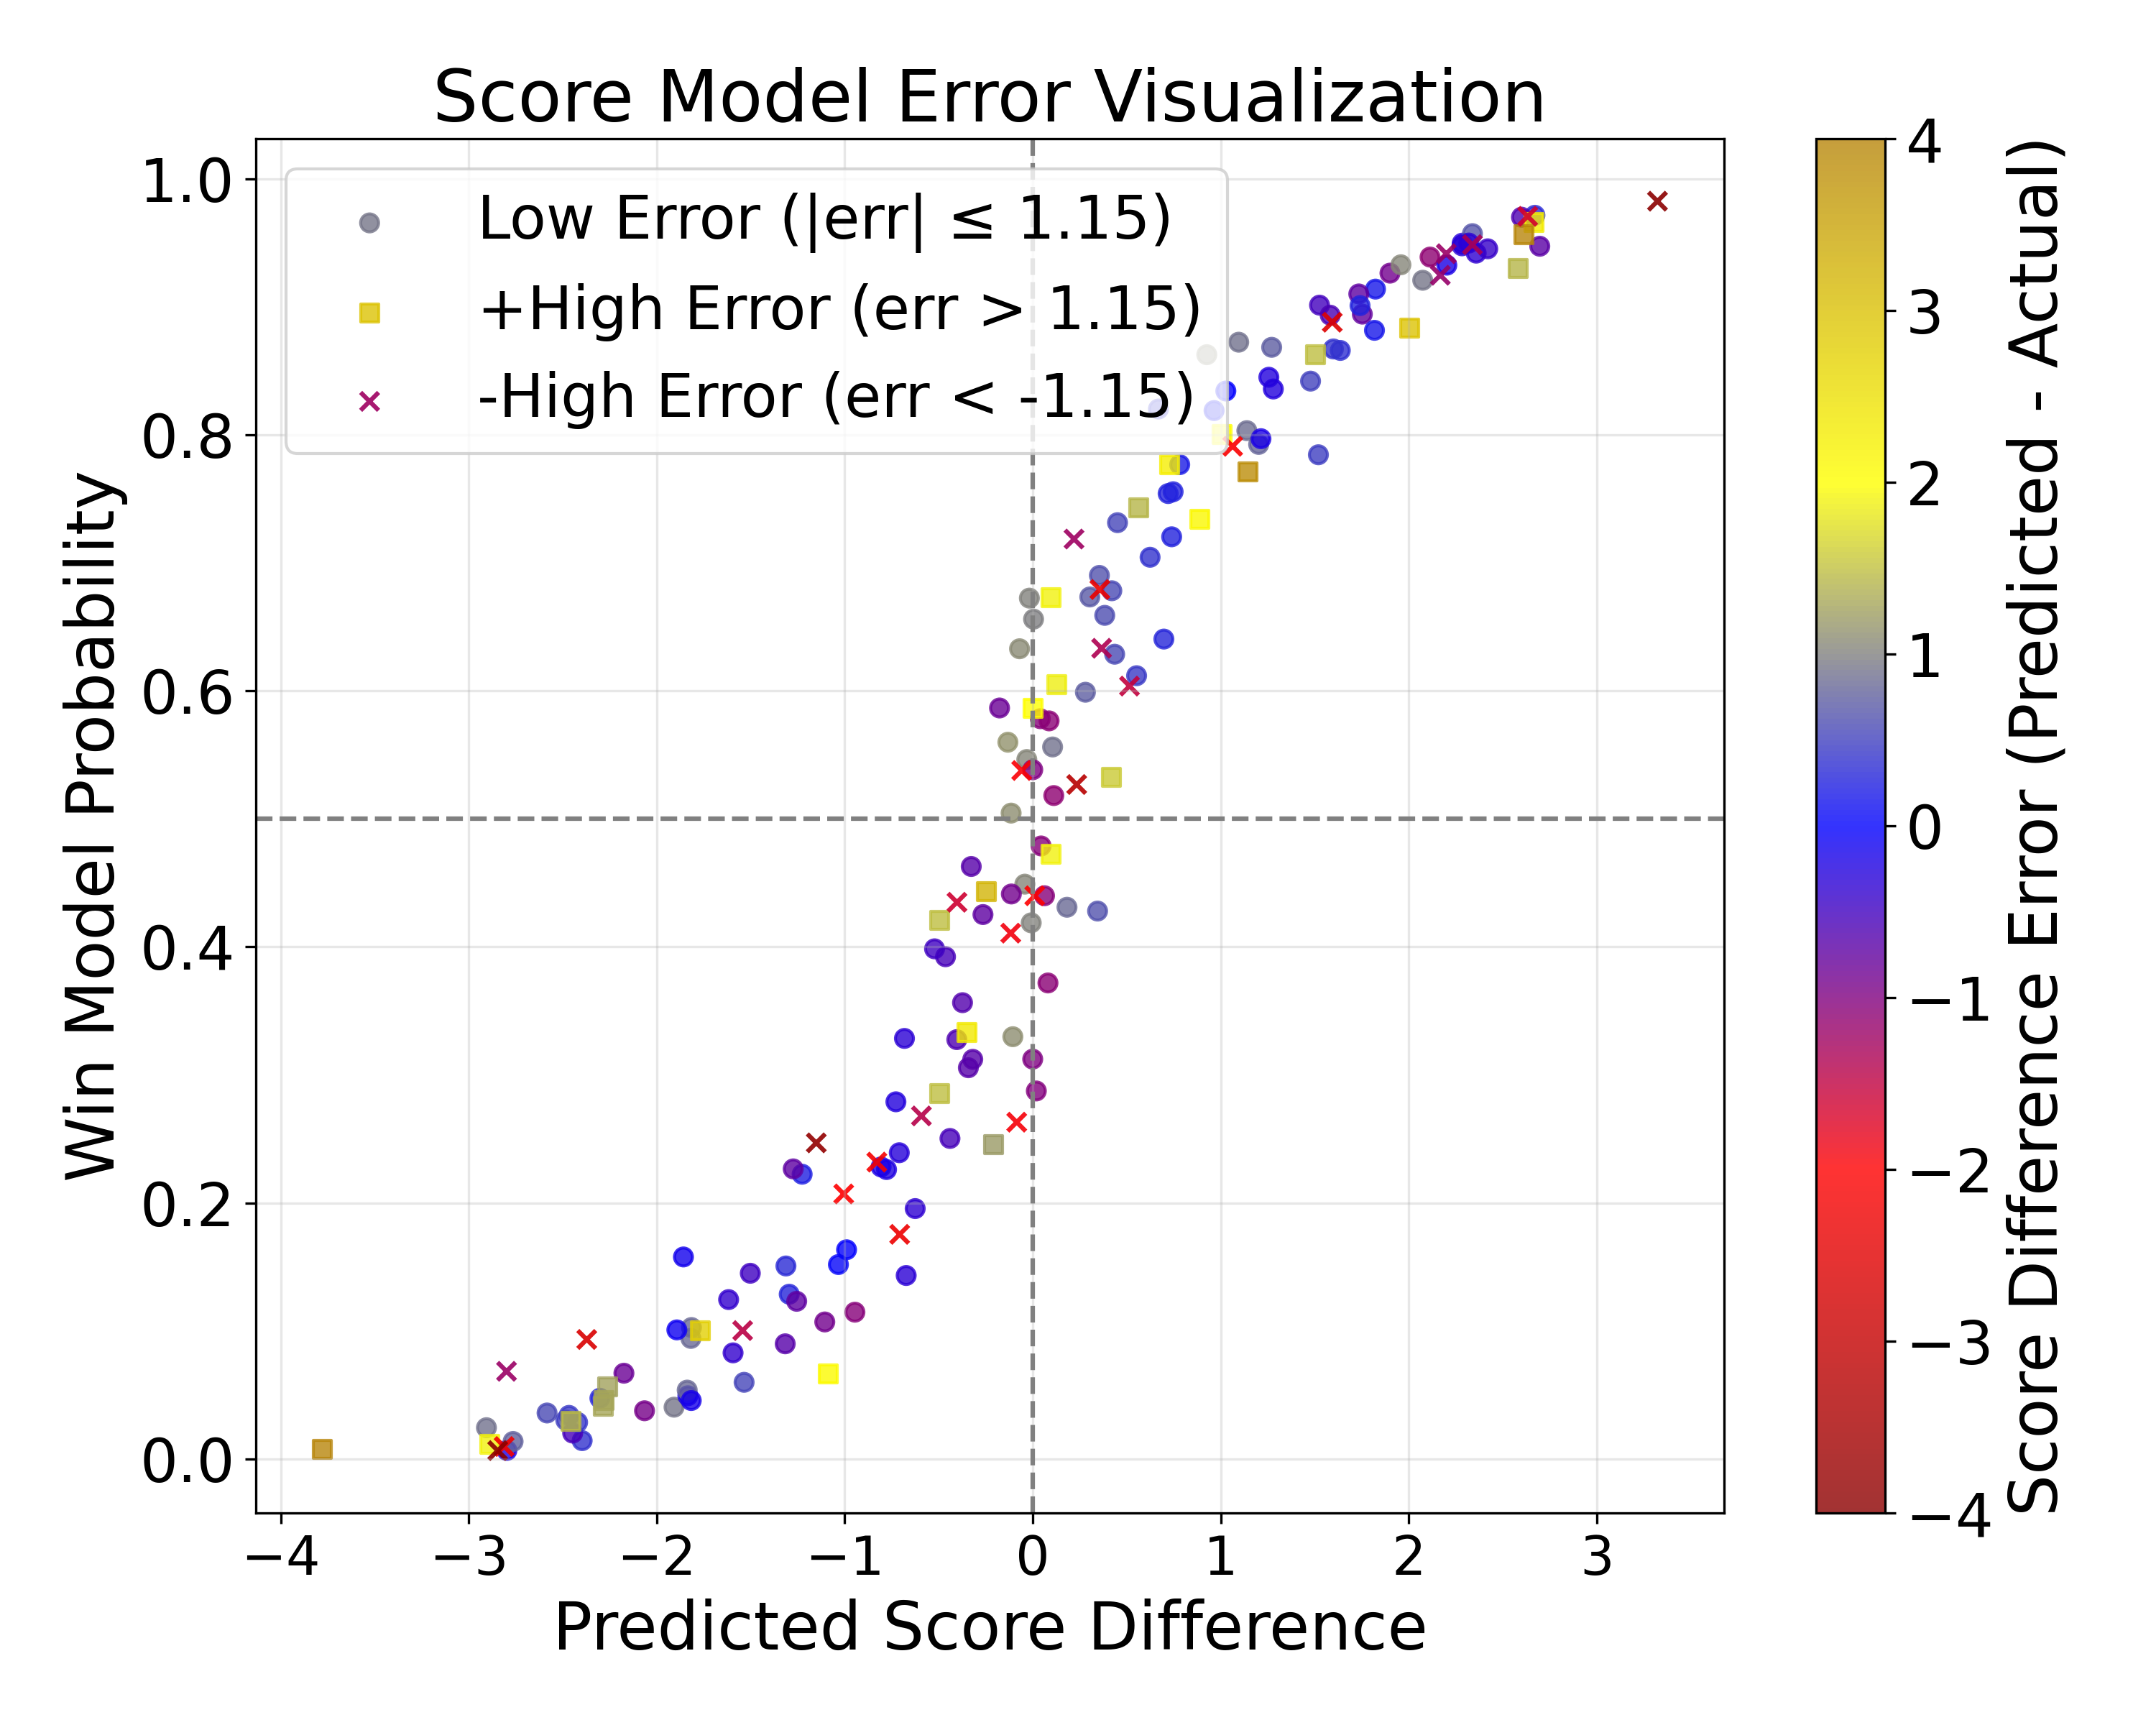
\includegraphics[width=0.85\linewidth]{Figures/4_score_error_graph.png}
  \caption{Score model error visualisation. Near-zero errors ($|\text{err}| \leq 1.15$ goals) are shown as blue circles; large positive errors (model underestimates) as yellow squares; large negative errors (model overestimates) as purple crosses. The colour gradient maps error magnitude from $-4$ to $+4$ goals.}
  \label{fig:score_error}
\end{figure}

\noindent
The majority of predictions (blue circles) fall within 1.15 goals of the actual outcome, with errors uniformly distributed across the predicted score range.
Large errors occur predominantly at the extremes of predicted advantage, where the model forecasts decisive victories that occasionally fail to materialise (purple crosses in the upper-right quadrant) or underestimates blowout results (yellow squares in the lower-left quadrant).
Critically, no systematic bias is visible: the error distribution is approximately centred at zero across all regions of the prediction space.

\subsection{Feature Importance Across Model Types}

Figure~\ref{fig:feature_importance} compares feature inclusion frequency in the top 20 models for both linear and neural network architectures.

\begin{figure}[H]
  \centering
  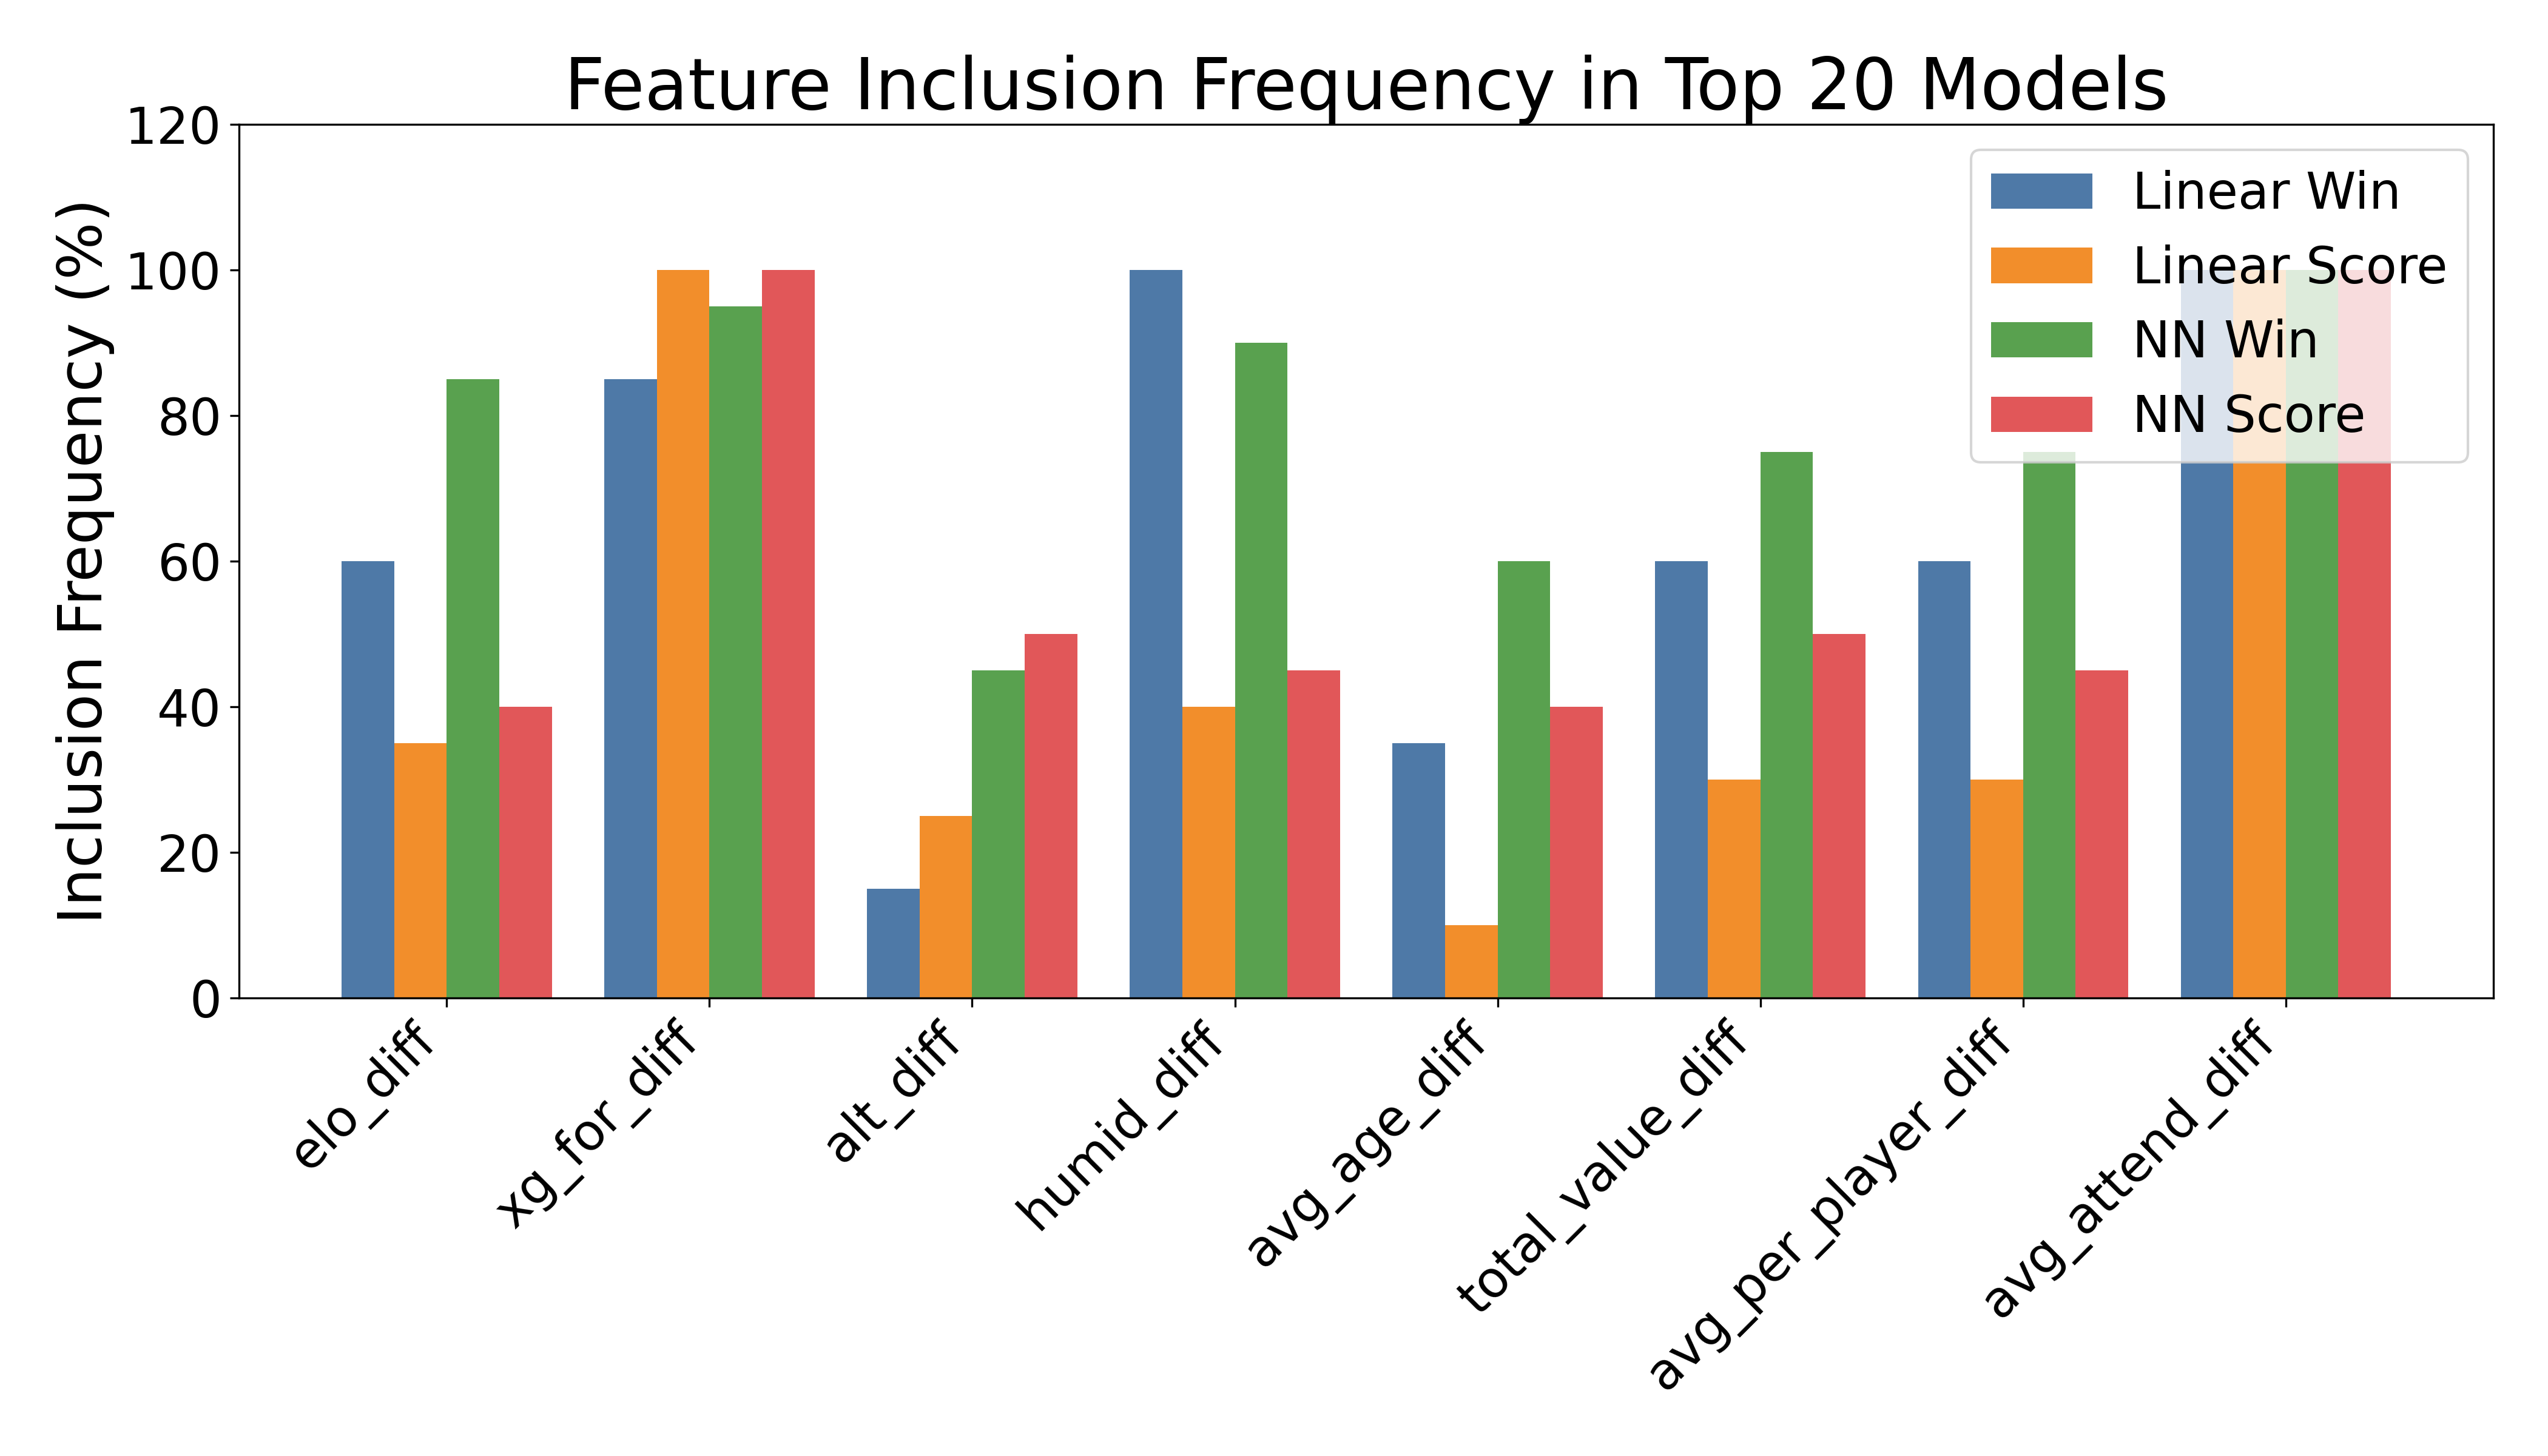
\includegraphics[width=\linewidth]{Figures/feature_importance_4models.png}
  \caption{Feature inclusion frequency in the top 20 models, comparing linear models and neural networks for both tasks. $\Delta$xG\textsubscript{for} and $\Delta$AvgAttend appear in nearly 100\% of top-performing models across all four configurations.}
  \label{fig:feature_importance}
\end{figure}

\noindent
Two features -- $\Delta$xG\textsubscript{for} and $\Delta$AvgAttend -- appear in 100\% of top-performing models regardless of model type or prediction task, establishing them as universally essential predictors.
$\Delta$Humid shows a pronounced task-specific pattern: it is present in 100\% of top linear win models and 90\% of top neural network win models, but drops to $\leq$~50\% for score prediction, confirming that humidity primarily influences match outcome direction rather than margin.
$\Delta$AvgAge and $\Delta$Alt exhibit the lowest inclusion rates across all four configurations, consistent with their negligible SHAP contributions.

\subsection{Sensitivity Analysis}

Figure~\ref{fig:sensitivity} presents partial dependence curves contrasting a strong feature ($\Delta$AvgAttend) against a weak feature ($\Delta$Alt) for the win classifier.

\begin{figure}[H]
  \centering
  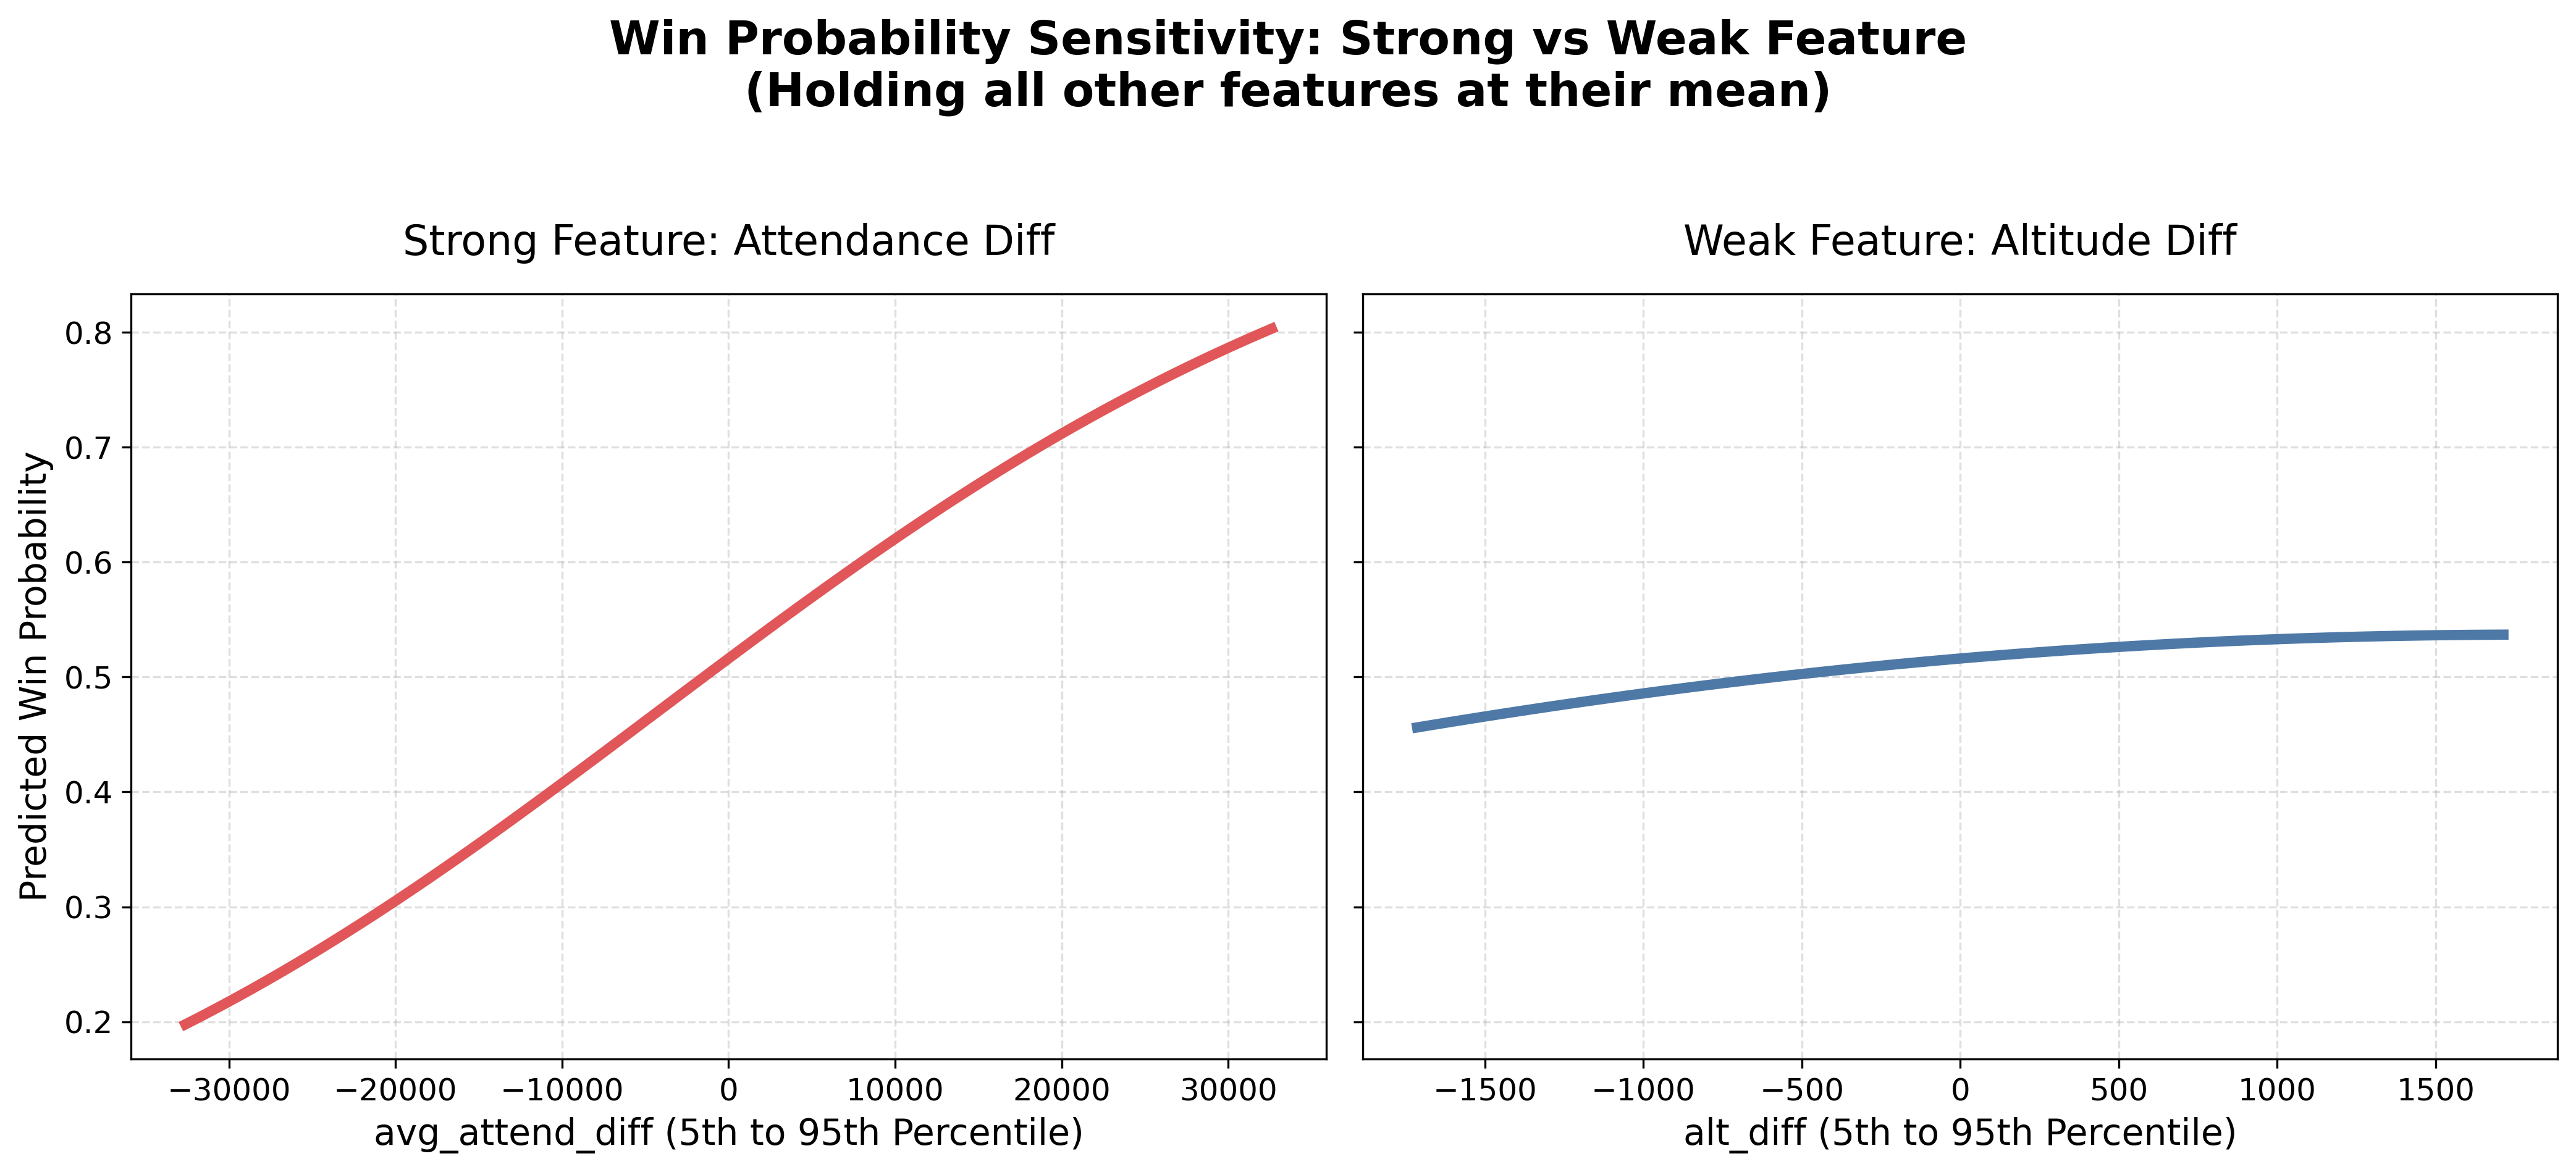
\includegraphics[width=\linewidth]{Figures/sensitivity_strong_vs_weak.png}
  \caption{Partial dependence (sensitivity) curves for the win classifier, sweeping each feature from its 5th to 95th percentile while holding all others at their mean. \textbf{Left:} $\Delta$AvgAttend produces a steep, near-linear response spanning 20--80\% win probability. \textbf{Right:} $\Delta$Alt produces a nearly flat response (45--54\%), confirming negligible marginal influence.}
  \label{fig:sensitivity}
\end{figure}

\noindent
The attendance differential sweeps win probability from approximately 20\% at its 5th percentile ($\Delta$AvgAttend $\approx -30{,}000$) to 80\% at its 95th percentile ($\Delta$AvgAttend $\approx +30{,}000$), a 60 percentage-point range.
By contrast, the altitude differential produces a nearly flat response across its entire range, varying win probability by fewer than 10 percentage points.
This quantitative contrast provides a direct, interpretable measure of relative feature influence beyond the aggregate statistics reported by SHAP.



% =====================================================================
%  4. DISCUSSION
% =====================================================================
\section{\uppercase{Discussion}}
\label{sec:discussion}

\noindent
The experimental results presented above yield several insights into the structure of international football prediction, the role of feature engineering, and the practical limits of model complexity on small datasets.
This section contextualises these findings against the prior literature and examines their broader implications.

\subsection{Attendance as a Latent Indicator of Institutional Quality}

The single most unexpected finding of this study is the dominance of stadium attendance difference as a predictor.
When used in isolation, $\Delta$AvgAttend achieves 82.0\% win classification accuracy -- surpassing both Elo (78.1\%) and Expected Goals (77.8\%) -- and ranks first in R$^{2}$ for score regression (Table~\ref{tab:single_feature}).
This feature appears in 100\% of top-performing models across all four model--task combinations (Figure~\ref{fig:feature_importance}), and the SHAP analysis identifies it as a co-dominant feature alongside $\Delta$xG\textsubscript{for} (Figure~\ref{fig:shap}).

We interpret this result not as evidence that crowd noise directly causes victories, but rather that average home attendance serves as a composite proxy for several correlated institutional factors: domestic league competitiveness, commercial revenue and infrastructure investment, supporter engagement, and the depth of the national footballing ecosystem.
A federation that consistently fills large stadiums is likely to possess stronger youth development, better coaching infrastructure, and higher overall squad quality -- attributes that are only partially captured by Elo or xG.
Mead et al.\ \cite{mead_expected_2023} have previously identified attendance as a contextual factor influencing shot conversion rates, and our results extend this observation from a match-level to a team-level predictive signal.

The sensitivity analysis (Figure~\ref{fig:sensitivity}) reinforces this interpretation quantitatively: sweeping $\Delta$AvgAttend from its 5th to 95th percentile shifts predicted win probability by 60 percentage points, while the same sweep for altitude -- a feature with an established physiological mechanism \cite{shephard_altitude_2008} -- produces fewer than 10 percentage points of variation.
This disparity suggests that in the context of World Cup football, even when teams are gathered from very different environments, other factors dominate such that the altitude advantage documented in domestic South American football is substantially attenuated.

\subsection{The Classification--Regression Divergence}

A central empirical finding is the opposing relationship between feature dimensionality and model performance for the two tasks.
Win classification accuracy increases monotonically from one to six features, levelling off around seven, while score regression peaks at two or three features and degrades with further additions.
This divergence is consistent with the theoretical framework proposed by Pitso et al.\ \cite{pitso_bayesian_2026}, who estimate that approximately 70\% of predictive uncertainty in football is aleatoric -- inherent randomness that cannot be reduced by model improvements or additional data.

For classification, the decision boundary between win and not-win is relatively coarse: it asks only whether the sum of advantages favours one side.
Additional features that are individually noisy (e.g., $\Delta$Humid with 50.2\% solo accuracy) can still contribute when combined with stronger predictors, because the classifier need only determine the \textit{sign} of the overall advantage.
The neural network's ability to learn non-linear interactions among these features explains the additional 1.0 percentage-point gain over the linear baseline (87.4\% vs 86.4\%).

For regression, the target is a continuous value (goal difference) that is subject to the full force of match-level stochasticity -- penalties, red cards, deflections, and goalkeeper errors can each shift the outcome by one or more goals independently of pre-match features.
Adding noisy features to the regression model increases the number of parameters that must be estimated from a fixed 256-observation sample, and the resulting overfitting manifests as degraded out-of-sample R$^{2}$.
The optimal three-feature neural network achieves R$^{2}$~=~52.0\%, implying that just over half of the variance in goal difference is captured by $\Delta$xG\textsubscript{for}, $\Delta$AvgPerPlayer, and $\Delta$AvgAttend; the remaining 48\% is attributable to match-level randomness that no pre-match feature can resolve.

\subsection{Architecture Simplicity and the Small-Data Regime}

Both final models employ single-hidden-layer architectures -- 32 units for classification and 16 for regression -- with no configuration deeper than one hidden layer outperforming these minimal topologies during the 64-configuration search.
This outcome is a direct consequence of the sample size constraint: with only 256 augmented training observations (128 original matches plus their mirrors), deeper networks rapidly overfit despite dropout and L$_{2}$ regularisation.

The choice of Swish activation over ReLU and Leaky ReLU (the other two candidates in the search) is empirically validated by the architecture comparison results.
Swish-based architectures consistently occupy the top positions in both tasks, likely because the smooth, non-monotonic gradient of Swish provides more stable optimisation in the low-data regime compared to the sharp zero-gradient region of ReLU.

The divergence in regularisation strength between the two models -- L$_{2}$~=~$10^{-4}$ for the classifier versus L$_{2}$~=~$10^{-3}$ for the regressor -- further reflects the classification--regression contrast.
The classifier, operating on seven features with a coarser decision target, benefits from lighter regularisation that preserves representational capacity.
The regressor, operating on three features with a noisier target, requires ten times stronger weight decay to prevent overfitting.

\subsection{Cross-Tournament Robustness}

The 86.8\% cross-tournament accuracy for win classification is a strong result in the context of international football prediction.
Tsokos et al.\ \cite{tsokos_modeling_2019} emphasise that temporal validation is the only methodologically sound approach for sports prediction, yet many published systems report only cross-validated accuracy on pooled data, which inflates estimates by allowing leakage of tournament-specific patterns.
Our 2018$\to$2022 testing protocol eliminates this source of optimism bias entirely.

The less than one percentage-point drop from 87.4\% (in-sample) to 86.8\% (cross-tournament) for win classification indicates that the seven selected features capture stable structural properties of international football rather than tournament-specific artefacts.
Elo ratings and xG are inherently forward-looking metrics that update between tournaments, attendance reflects durable institutional characteristics, and market values track slow-moving talent pipelines -- all of which change gradually rather than abruptly.

The more substantial R$^{2}$ decline for score regression (52.0\% $\to$ 39.8\%) is expected: exact goal margins are more sensitive to tournament-specific factors such as officiating standards, ball characteristics, and climate conditions that differ markedly between Russia (2018) and Qatar (2022).
Despite this decline, the cross-tournament R$^{2}$ remains close to the linear in-sample baseline, confirming that the neural network's superior in-sample performance stems from genuine signal extraction rather than overfitting.

\subsection{Fault Analysis Thresholds}

A critical operational question for any predictive system is the determination of a fault analysis threshold: at what point of deviation between the predicted and actual outcome should the model flag a ``fault'' or anomaly for further investigation? Based on our empirical results, a reasonable heuristic is to flag a match when the actual goal difference deviates from the prediction by more than 1.0 Mean Absolute Error (MAE). Given our regression baseline MAE of 1.055, an error exceeding this magnitude suggests that the match outcome was influenced by factors significantly outside the model's expected variance, warranting a deeper analysis of the match events. However, the precise calibration of this threshold requires further research to balance the rates of false positives and false negatives. This approach aligns with established practices in anomaly detection across other domains; for instance, Hundman et al.\ \cite{hundman_detecting_2018} have demonstrated the utility of using prediction error thresholds for detecting anomalies in complex systems, establishing that errors exceeding baseline metrics serve as robust indicators of system deviations.

\subsection{Limitations}

Several limitations should be acknowledged.
First, the training sample comprises only 128 unique matches (64 per tournament), which restricts the model's ability to learn complex interactions and limits the reliability of significance testing.
Second, the binary classification formulation treats draws as non-wins, collapsing a three-class problem into a two-class one; future work could adopt ordinal regression or a three-way classifier to preserve draw information.
Third, the feature set relies on pre-tournament aggregate statistics and does not incorporate match-day dynamic variables such as injuries, tactical formations, or in-match momentum shifts, which are known to influence outcomes.
Fourth, the evaluation is limited to FIFA World Cup matches and may not generalise to other tournament formats (e.g., continental championships or domestic leagues) where team quality distributions and match conditions differ.
Finally, while the SHAP analysis provides local interpretability, it does not capture interaction effects between features, which may be important given the non-linear nature of the neural network models.


% =====================================================================
%  5. CONCLUSIONS
% =====================================================================
\section{\uppercase{Conclusions}}
\label{sec:conclusion}

\noindent
This paper has presented a systematic prediction pipeline for international football, proceeding from feature engineering through exhaustive combinatorial selection to neural network architecture optimisation, evaluated under strict cross-tournament temporal conditions on the 2018 and 2022 FIFA World Cups.

The analysis yields three principal conclusions.
First, the exhaustive combinatorial search reveals a fundamental divergence between classification and regression in low-scoring sports: win prediction benefits from rich, multi-source feature sets (seven features, 87.4\% accuracy), while score-margin estimation requires aggressive feature reduction (three features, R$^{2}$~=~52.0\%) to avoid overfitting to aleatoric noise.
This divergence provides empirical support for the theoretical finding of Pitso et al.\ \cite{pitso_bayesian_2026} that the majority of uncertainty in football outcomes is irreducible.

Second, stadium attendance difference emerges as the single most powerful individual predictor of both win probability and score margin, outperforming established metrics including Elo ratings and Expected Goals when used in isolation.
This finding identifies attendance as a previously underutilised composite indicator of institutional footballing quality and warrants further investigation across broader datasets and competition formats.

Third, the selected feature-architecture pairings demonstrate strong temporal generalisation, with win classification accuracy degrading by less than one percentage point across a four-year gap between training and test tournaments.
This robustness is attributable to the deliberate construction of features from slowly evolving institutional and performance indicators rather than transient match-level statistics.

Future work should extend this framework in several directions: (i)~expanding the dataset to include continental championships and qualification rounds to increase sample size and diversity; (ii)~incorporating match-day dynamic features such as tactical formations, real-time injury reports, and in-play momentum indicators; (iii)~adopting three-class ordinal regression to model draws explicitly; and (iv)~investigating ensemble methods that combine the classification and regression outputs into a unified probabilistic forecast.


\bibliographystyle{apalike}
{\small
\bibliography{references}}


\end{document}